\documentclass[12pt]{article}
\usepackage[utf8]{inputenc}
\usepackage{enumitem}
\usepackage{graphicx}
\usepackage[margin=1in]{geometry}
\usepackage{amsmath}
\usepackage{amssymb}
\usepackage{mathtools}
\usepackage{authblk}
\usepackage{hyperref}
\usepackage[ruled,vlined]{algorithm2e}
%\setlength{\parskip}{1em}
\title{Unique Component Analysis}
\author[1]{Robin Tu}
\author[2]{ Alexander H. Foss }
\author[1]{Sihai Dave Zhao}
\affil[1]{Department of Statistics, University of Illinois at Urbana-Champaign, Champaign, IL}
\affil[2]{Statistical Sciences, Sandia National Laboratories, Albuquerque, NM}

%\date{August 2020}

\begin{document}

\maketitle

\section{Introduction}
Dimension reduction for high-dimensional data visualization and exploration is an universal problem across many disciplines. %(more and more frequent. people are using these methods more) 
%One way of visualizing high dimensions is to employ a dimension reduction method which would embed high-dimensional relationships in a dimension humanly digestible. There is a rich literature which focuses on dimension reduction on a single data set for almost every situation imaginable.
For continuous data, methods include Principal Component Analysis (PCA \cite{pca}), Nonnegative Matrix Factorization \cite{Lee1999}, Projection Pursuit \cite{pp}, Independent Component Analysis (ICA \cite{ica}), with newer nonlinear techniques such as t-SNE and UMAP gaining popularity in the field of bioinformatics [CITATION??]. % Research on dimension reduction on a single numeric dataset for almost every situation imaginable have been published on extensively.  These include: PCA, .. , ICA with newer non-linear techniques gaining popularity in the field of bioinformatics.
% Challenges which arose from applying dimension reduction methods developed specifically for continuous data onto nonstandard, nonnumerical, and mixed-type data were addressed with methods like Multiple Correspondance Analysis (MCA), Extending PCA (XPCA \cite{xpca}), and Factor Analysis for Mixed Data \cite{famd}(FAMD), respectively.
%This arsenal of techniques satisfy most dimension reduction situations researchers encounter. 

However, data is universally plagued by biological and/or technical variability which reduce the effectiveness of dimension reduction methods to find meaningful latent structure/variables. To handle these sources of variation, vast problem specific (sometimes technology specific: methylation 450k vs 850k) pipelines have been established to remove experimental artifacts such as batch effects (batch normalization), inherent within sample variation, and correct for machine/data generating error \cite{Nguyen2019}. These pipelines sometimes make assumptions about the data generating process, such as removing top principal components (PCs) due to mostly comprising of noise, possibly discarding relevant information. This is especially problematic in high-dimensions, with limited samples.

%Even the number of PCs microarray data exists in is contested  \cite{rpca}.

Contrastive methods are a recently developed class of procedures for simultaneously removing unwanted variation while performing dimension reduction. By leveraging a background dataset that represents unwanted or known variation, contrastive methods seek to model or explain variation unique to the target data of interest, variation which doesn't exist in the background. There are many other types of contrastive implementations including latent models  \cite{severson2019unsupervised} and autoencoders  \cite{cautoencoder}, but we focus on dimension reduction for continuous data types, specifically contrastive PCA \cite{Abid}.
%Within dimension reduction, there are of the continuous (contrastive PCA \cite{Abid}) and categorical flavor (contrastive MCA  \cite{fujiwaraMCA}).


%\begin{enumerate}
%    \item residual PCA  \cite{rpca}
%        \begin{enumerate}
%            \item projecting data into the space span by the eigenvectors associated with the smallest $p-k$ eigenvalues of the background data
%            \item assumes that background data exists in low dimensional space
%            \item still requires tuning number of dimensions $k$ that encompasses most of the background covariance
%        \end{enumerate}
        
   Abid et al introduced the contrastive methodology with contrastive PCA (cPCA) \cite{Abid}, which utilized a secondary background data set of known and unwanted variability to uncovered new unique directions of maximal variation in a target data.
   Let $A$ denoted the $p\times p$ sample covariance matrix constucted from target data $X_{n_x \times p}$ and $B$ denote the $p\times p$ sample background covariance constructed from background data $Y_{n_y \times p}$. For some contrastive parameter $\lambda$, cPCA seeks the eigenvectors $v$ satisfying \[\max_{v\in \mathbb{R}^p}v^T\left(A - \lambda B\right)v\] 
   resulting in eigenvectors which maximize variability in the target data, while simultaneously minimizing variability in the background data.
   The tuning parameter $\lambda$, which measures how much to penalize the background data covariance, greatly impacts the resulting eigenvectors. $\lambda = 0$ reduces cPCA to normal PCA since no weight is applied to the background data whereas a $\lambda \rightarrow \infty$ is equivalent to PCA after projecting the target data onto the nullspace of the background data.  The authors of cPCA suggested that $\lambda$ is chosen using spectral clustering via a parameter sweep of logarithmically spaced candidate values.

%    \item cPCA  \cite{Abid}
%        \begin{enumerate}
%            \item introduced contrastive framework to PCA
%            \item by subtracting the background data covariance from the target data covariance, they hoped to uncover directions of maximal variation unique to the target data alone.
%            \item if A denoted the target data covariance and B the background data covariance, Abid et al sought the eigenvectors which \[\max_{v}v^T\left(A - \alpha B\right)v\]
%            \item Abid et al. chose the tuning parameter $\alpha$ which measures how much to penalize the background data covariance,via a parameter sweep of 40 logarithmically spaced values between 0.1 and 1000. The best possible $\alpha$ values were chosen using spectral clustering.
%            \item since construction of target and background data covariance matrices are required, this method does not scale to higher dimensional data.
%        \end{enumerate}
     
     cPCA has already inspired several variants. Fujiwara et al.  \cite{Fujiwara} applied cPCA to identify variables most influential in maximally contrasting clusters by using the entire data as the target data, and the data of interest as the background. The authors suggest choosing $\lambda$ from a similar candidate set which maximize  the separation between the target cluster and all other data while still having enough variance in the target cluster K. % where a list of candidate $\alpha$ are evaluated based on distance between the target and background projections on the corresponding first contrastive principal component. 
    %\item ccPCA: Contrasting Clusters in PCA  \cite{Fujiwara}
    %\begin{enumerate}
    %    \item specific use case of cPCA to find the variables most influential in directions which maximally contrast clusters by letting the target be the clusters of interest and background be all other data points. 
    %    \item must choose the number of clusters first, and does 1-vs.-others comparison, 
    %    \item they put the entire dataset as the target data and use the "target of interest" as the background.
    %    \item propose an semi-automatic selection of $\alpha$ where a list of candidate $\alpha$ are evaluated based on distance between the target and background projections on the corresponding first contrastive principle component
    %    \item unable to solve the high dimensional problem with contrastive analysis
    %\end{enumerate}
    Salloum and Kuo  \cite{Salloum} introduced cPCA++, %motivated by image splicing localization, classifying whether a pixel belonged to the original image or an image splice. Using a generalized likelihood ratio test framework to test whether a pixel belonged to foreground or background, they arrived at a Rayleigh Quotient of target variation divided by background variation. Using similar notation as above where $A$ denotes the target sample covariance matrix and $B$ denotes the background sample covariance matrix, cPCA++ seeks to:
    where they seek to maximize the ratio, rather than the difference, of the variance explained in the target to the variance explained in the background.%\[
    %\max_{v \in \mathbb{R}^p} v^\top A v \mbox{ subject to } v^\top B v = 1.
    %\]
    %\[\max_{v\in \mathbb{R}^p} v^T\left( B^{-1} A\right) v\]
    %which does not require iterating through candidate contrastive parameters. This method uses a matrix inversion of a $p \times p$ background covariance matrix, which may be rank deficient, requiring the addition of some $\epsilon > 0$ onto the diagonal. The addition of $\epsilon$ onto the diagonal of the background matrix induces regularization depending on the choice of $\epsilon$, making this approach not exactly without tuning parameters.
    %The resulting eigenvectors can be shown to diagonalize the background matrix, ie $v^T Bv =1$, however, the eigenvectors are no longer orthonormal, ie $v^T v = I_p$. 
      %\item cPCA++: \cite{Salloum}
        %\begin{enumerate}
            %\item "No tuning" parameter: it's still there in the matrix inversion with the choice of $\epsilon$. note: by eigen decomp $B = VDV^{-1}$, then $(B+cI)^{-1} = (VDV^{-1} + VcIV^{-1})^{-1} = V(D+cI)^{-1}V^{-1}$ is similar to lasso
            %\item approach from a a Generalized Likelihood Ratio Test framework and arrived at a tuning free solution to cPCA using the Rayleigh Quotient.
            %\item  requires matrix inversion of $p\times p$ covariance matrix, which requires positive definiteness of the background covariance matrix.  If rank deficient they add $\epsilon$ to the diagonal of the background covariance matrix.
            %\item no constraints on  $v^T B v$ when solving the optimization $max_{v}{v^TB^{-1}Av}$ will find a solution where $v^T B v \approx 0$ and $v^T A v$ is not very large, but the rayleigh quotient still blows up. This means a suboptimal direction 
            %\item adding $\epsilon$ to the diagonal is sort of cheating because it adds regularization. it forces $v^T B v > \epsilon $. choosing $\epsilon$ is also a tuning parameter
            %\item the eigenvectors $v$ are no longer orthogonal, therefore directions found are correlated. Forget trying to 
            %\item no intuitive extension to multiple data
        %\end{enumerate}
Boileau et al.  \cite{Boileau} described Sparse cPCA (scPCA) by adding $l_1$ and $l_2$ penalties to sparsify the estimated eigenvectors of the contrastive covariance matrix. %As a consequence of introducing sparsity, the eigenvectors are no longer uncorrelated. 
    %Furthermore, scPCA requires taking the square root of a positive semi-definite
    %\item scPCA: several tuning parameters  \cite{Boileau}
    %\begin{enumerate}
    %    \item extend cPCA by using the framework in sparse PCA to sparsify the eigenvectors of the contrastive covariance matrix, $\boldsymbol{C}_\gamma$.
    %    \item adds additional $l_1$ and $l_2$ tuning parameters on top of the original contrastive tuning parameter, $\gamma$. To tune these, authors suggest a parameter sweep via clustering algorithm on the best combinations of $(\gamma, l_1)$.
    %    \item requires construction of the contrastive covariance matrix, which does not scale to higher dimensional data.
     %   \item requires taking the square root of $\boldsymbol{C}_\gamma$, the P.S.D contrastive covariance matrix, which may be rank deficient and require addition of $\epsilon$ on the diagonal or replacing negative eigenvalues with 0.
     %   \item eigenvectors are no longer uncorrelated
    %    \item no intuition on how to extend to multiple data
    %\end{enumerate}
   
   However, there are two main disadvantages to these existing methods. First, they cannot accommodate multiple background datasets. Multiple backgrounds would allow researchers to target the exact variability of interest by removing unwanted variation from multiple sources and/or conditions. For example...
   Naively applying existing methods by stacking the multiple background data matrices together and forming a pooled covariance matrix will not work well. The pooled covariance is a sample-weighted average of the individual background covariance matrices and may not be representative of any of the individual datasets. %The resulting best case scenario is multiple backgrounds with the exact same covariance matrix such that background variation is preserved.  However, the worst case scenario, background covariances may sum to a diagonal matrix, washing out background variation when stacking and reducing cPCA and its variants to PCA. 
   
   The second disadvantage of existing contrastive methods is that they require one (e.g., cPCA and ccPCA) or several (e.g., scPCA) tuning parameters, user input variables that influence an algorithm's behavior. Since existing contrastive methods heavily depend on the tuning parameter, finding the optimal tuning parameter(s) which balances the dual mandate of maximizing variability in the target and minimizing variability variability in the background may be tedious and frustrating. Although cPCA and ccPCA have criteria-based tuning parameter solutions, the right tuning parameter may not be among the default candidates. An apparent exception is cPCA++, but in practice it requires a tuning parameter when its background sample covariance matrix is not positive definite, which is common many applications.
   
   %Lastly, from a computational perspective, they each revolve around the construction of the complete $p \times p$ contrastive covariance matrix, involving two $p\times p$ target and background covariance matrice. When $p$ is large, the required memory scales with $p^2$, making these methods unsuitable for high-dimensional settings, especially for dense matrices.
    
    
    We propose Unique Component Analysis (UCA) to address both of these issues. UCA works by constraining the objective function in cPCA to give directions that are orthonormal and explain small amounts of variation in each background dataset. Specifically, let $A$ be the $p \times p$ target covariance matrix and $B_j$, $j \in 1,...,m$ be the $m$ $p\times p$ background covariance matrices. We seek to: 
     \begin{align}
         &\max_{v\in \mathbb{R}^p}{v^TAv} \nonumber\\ 
         \text{subject to }&\; v^{T}v=I,\;\; v^TB_1 v \leq 1, \cdots, v^T B_m v \leq 1 \nonumber
     \end{align}
    These constraints are naturally found in generalized eigenvalue problems and can be solved using weak duality of the Lagrangian.
    UCA is tuning-free, is easily extensible to multiple background data sets, and is scalable to high-dimensions. We hope to provide a way for researchers to explore higher dimensional data and uncover variation unique to the data of interest, variation not shown in previous studies, control groups, and other known sources of variation, simultaneously. UCA seeks to find the unique directions of variation which both maximize the varability in the target dataset and also account for little variation in each of the background dataset(s). We show that UCA achieves similar results as cPCA and cPCA++ with a single background dataset and that it can outperform them when using multiple backgrounds. %We then use UCA to find prominent emotional features using eigenfaces and illustrate where stacking may fail. In the methods section, we provide detail to how UCA works and how we handle high-dimensional problems. 
    %We provide three examples illustrating the effectiveness of UCA and 

Another way to conduct contrastive dimension reduction is with ``Residual PCA''. We note that residual PCA (rPCA) is not a formal technique but is used as an ad-hoc method of removing noise from known variability  \cite{rpca}. Again, let $A$ be the $p \times p$ target covariance matrix and $B$ be the $p\times p$ background covariance matrix.  For some integer $k$ which denotes the low dimensional representation of $B$, rPCA performs PCA after projecting $A$ onto the ``residual'' space of $B$. More specifically, if $W$ denotes the eigenvectors of $B$ and $W_{(k+1):p}$ the top $(k+1):p$ eigenvectors of $B$,then rPCA seeks to:
\[\max_{v\in \mathbb{R}^p}{v^T \left(W_{(k+1):p}W_{(k+1):p}^T A\right) v}\]
Note that cPCA with contrastive parameter $\lambda \rightarrow \infty$ is different from rPCA because rPCA requires user to choose the number of background components to be kept, whereas cPCA with $\lambda \rightarrow \infty$ maps reduces the target on the nullspace of the background-- they would be equivalent for $k = p$. We present rPCA to demonstrate that some of the same underlying directions can be found in a more intuitive way. It also can easily be extensible to multiple backgrounds by projecting onto addition background residual spaces. Since the residual space of the background can be done easily with singular-value decomposition, it is computationally simple and straight forward. However, one still needs to choose the background data dimension, $k$.
To solve this tuning parameter problem, we use the elbow method of finding the best linear single knot spline at $k$ such that the mean-square error is minimized in the scree plot.%(Cite...I don't remember the citation for this...)
   
   
   
\section{Results}
\subsection{Subgroup discovery in protein expression data}
The goal of the mouse protein expression experiment was to assess whether Memantine recovered the ability to learn in Down Syndrome mice, with the aim to identify subsets of protein that discriminate between treatment classes.
 The study measured expression of 76 mice proteins of 1080 control or trisomic (Down Syndrome) mice samples (each mice measurement considered an independent sample/mouse), which received a combination of shock therapy (Context Shock vs. Shock Context) and drugs (Saline vs. Memantine)  \cite{Ahmed, Higuera, Abid}.  
Since saline treated mice not exposed to shock therapy (Shock Context) are similar to those that are saline treated but also exposed (Context Shock) to shock therapy, we can investigate the variation unique to undruged and unshocked mice by contrasting shocked control mice protein expression measurements, which removes variation resulting from shock therapy. Doing so may show how control mice and Down Syndrome mice differ in the control setting.
We compare the principal directions found by UCA to those found by PCA, cPCA ($\lambda = 0.5, 1, 5, 10$), cPCA++, and rPCA on Saline injected mice which have not received shock therapy (Shock Context) and use Down Syndrome class to evaluate separability when observations are projected onto the first two directions found by each method.

The results in Figure \ref{fig:Mouse} show that PCA has difficulty distinguishing between mice with Down Syndrome and mice without.  In this example, the resulting separation in the first two contrastive principal components does not depend on the chosen $\lambda$. At all values of $\lambda$, cPCA achieves good separation, therefore it is unsurprising UCA has similar results. These results align with the results found in  \cite{Abid}.
cPCA++, which also does not require specifying a contrastive tuning parameter, performs better than PCA at separating control and Down Syndrome mice, but falls short of achieving similar performance to cPCA for any value of the contrastive tuning parameter. Interestingly, the simple and intuitive rPCA method, with $k$ chosen by single knot spline with smallest MSE, achieved similar results to both cPCA and UCA, while outperforming cPCA++.

% rewrite caption
\cite{Abid} we confirm their results. 
\begin{figure}[t]
    \centering
	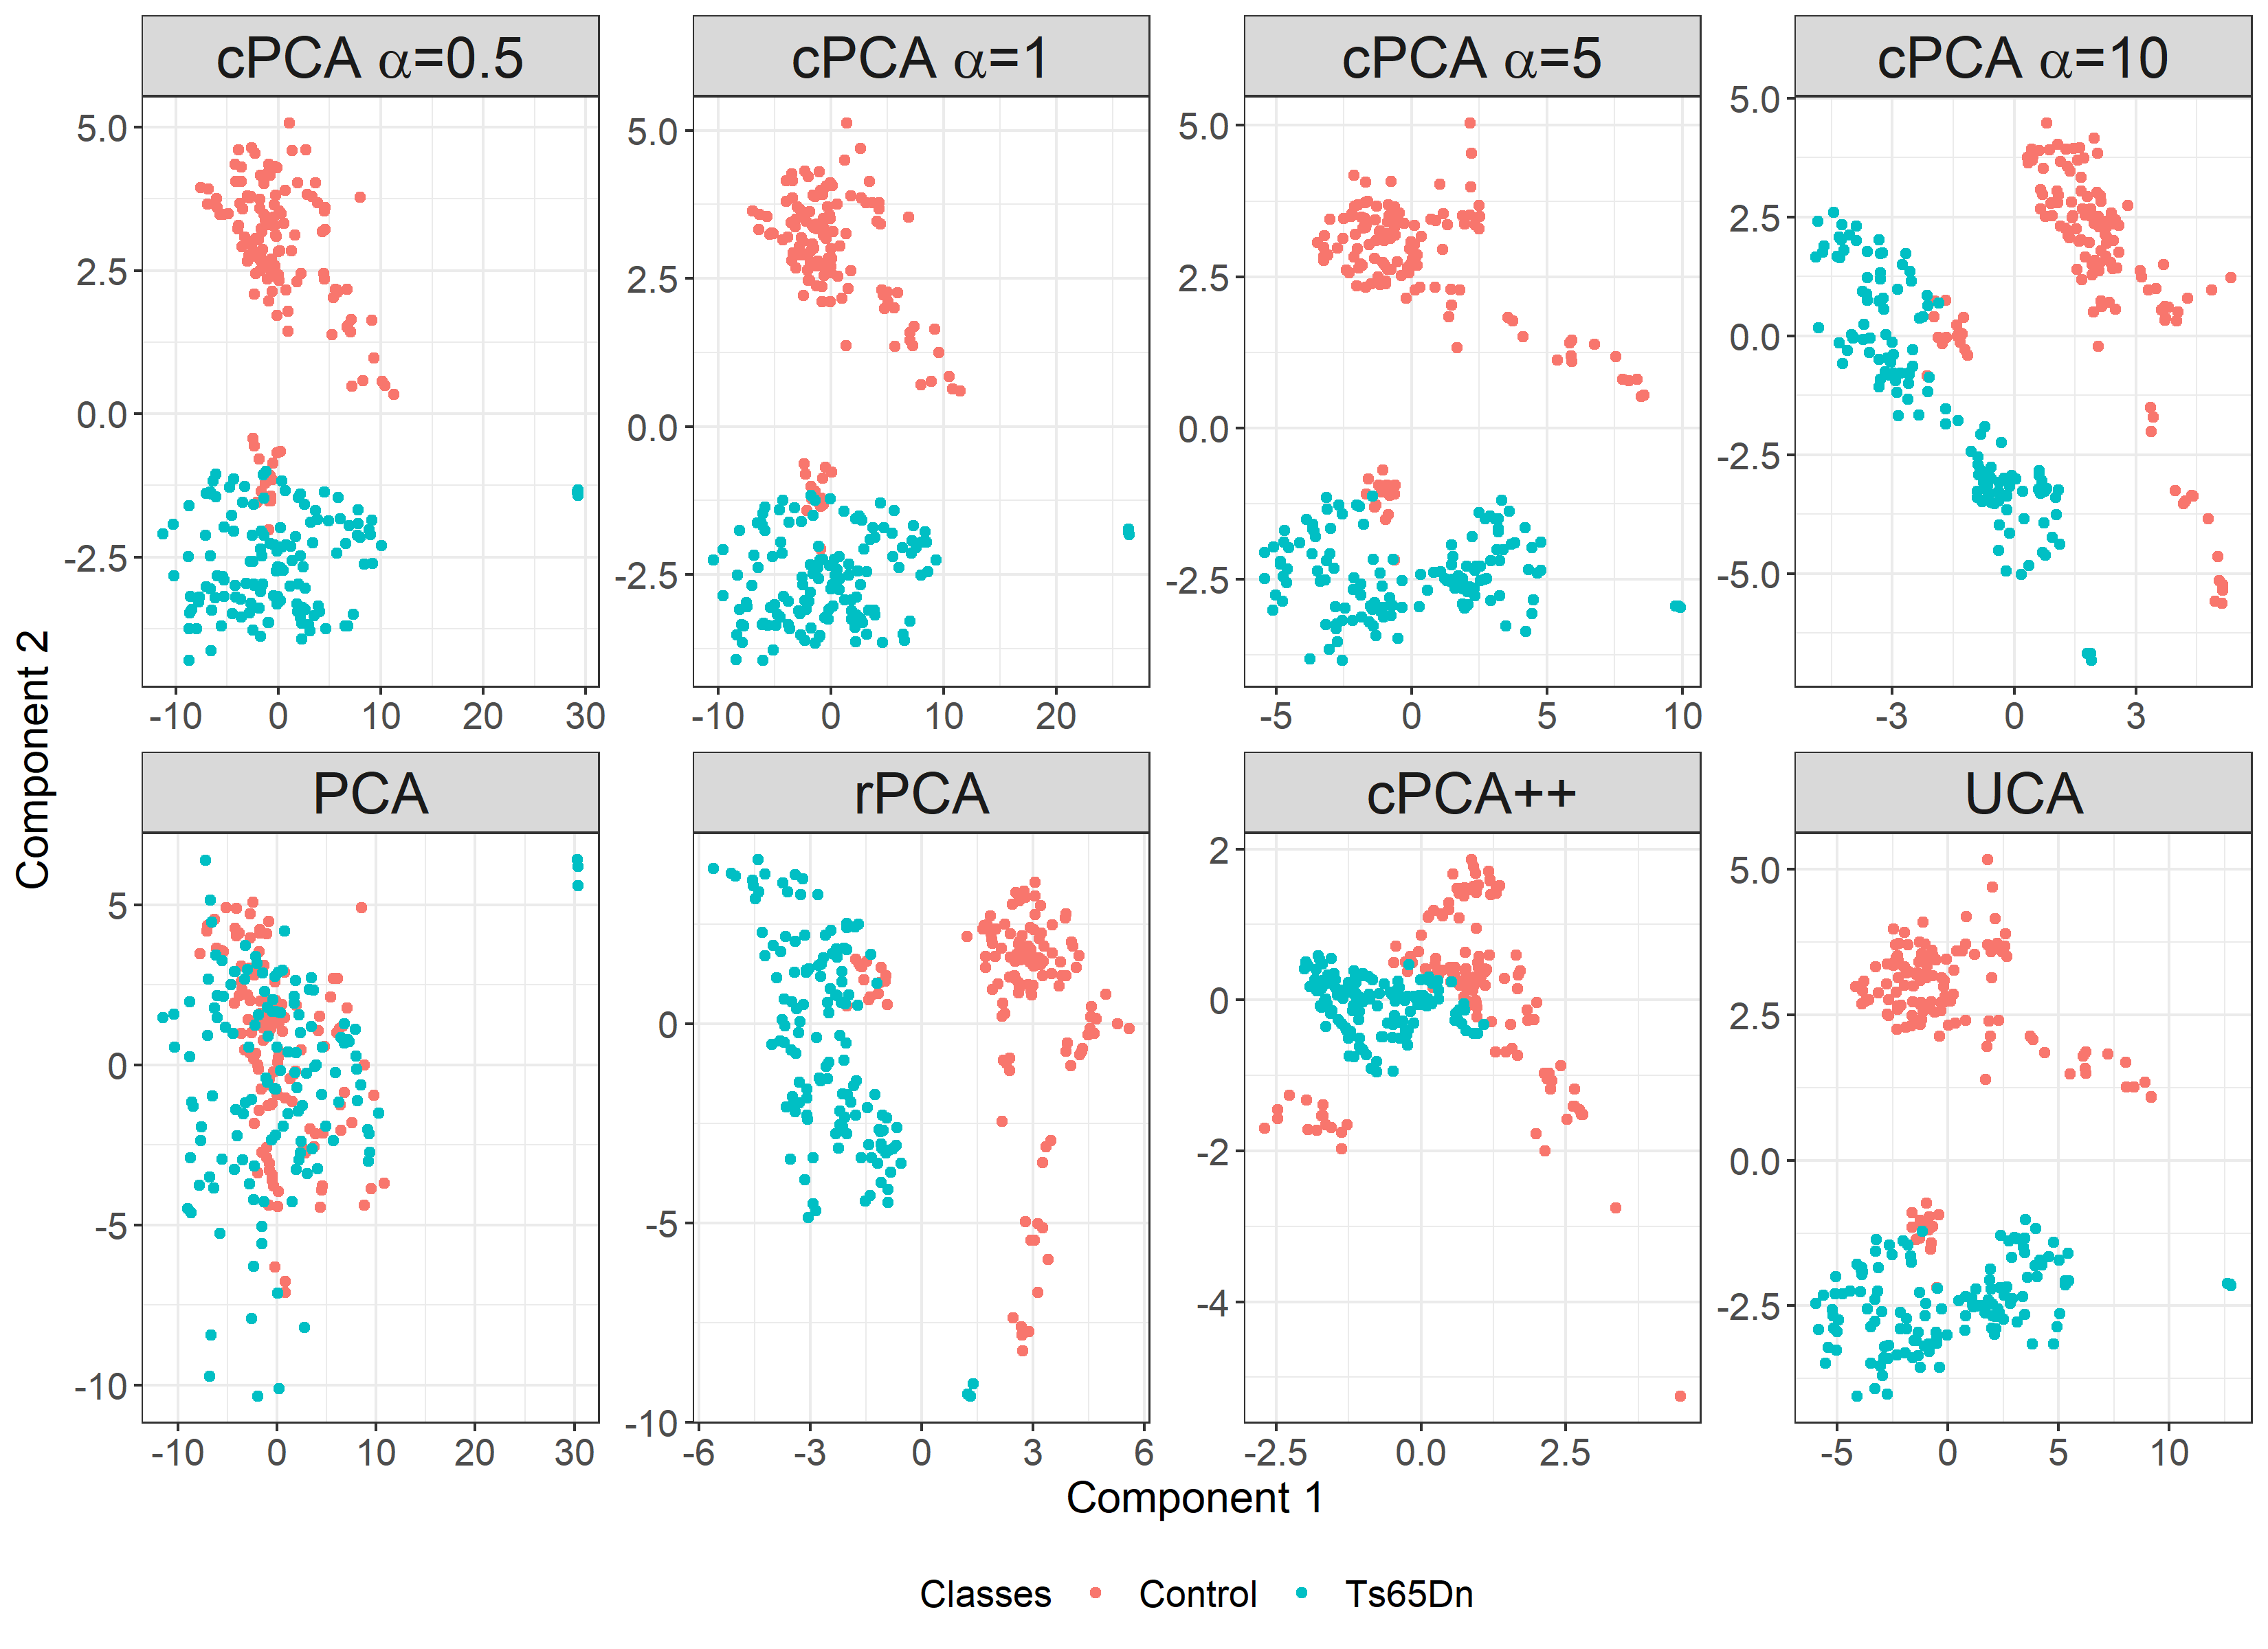
\includegraphics[width = 0.8\textwidth]{figure/Mouse_Data.png}
	\caption{Mouse Protein Expression: Separability of Saline injected mice which were not shocked. confirming  \cite{Abid} results where a background of Saline injected mice who were shocked was used. This example is unseparable using PCA alone but is easily separable by cPCA for all values of $\alpha$, cPCA++, rPCA, and UCA.}
	\label{fig:Mouse}
\end{figure}

\subsection{Subgroup discovery in protein expression data with multiple backgrounds}
A more challenging problem for cPCA and it's variants is separating Down Syndrome and Control mice when the target involves Saline injected mice which received shock therapy. In figure \ref{fig:MouseSplitStack} we show the results of PCA, cPCA++, rPCA, and UCA with a variety of backgrounds (shown in parenthesis): memantine injected mice with Down Syndrome that were shocked (Mem-C/S-Ts65Dn), memantine injected mice with Down Syndrome that were not shocked (Mem-S/C-Ts65Dn), saline injected mice with Down Syndrome that were not shocked (Saline-S/C-Ts65Dn), all of the aforementioned backgrounds stacked before forming their joint covariance matrix (Stack All), and aforementioned backgrounds treated as separate backgrounds simultaneously (Split All). 

PCA and the single background condition UCA, cPCA++ and rPCA ($k$ chosen with single knot spline with lowest MSE) with stacked background cannot distinguish between Down Syndrome and control mice. UCA with stacked background performs better at splitting the two groups compared with the other methods.  However, UCA with split background yields almost complete separability compared with the stack background result, demonstrating the additional leverage when we treat each background separately.
We note that this problem isn't easily separable by using cPCA++, rPCA, and cPCA with a variety of contrastive parameter and the results are generally worse than figure \ref{fig:MouseSplitStack} (see figure \ref{fig:mouse_stack_cpca} in the Appendix). 

%We also note that the choice of background is crucial and that not some backgrounds are unsuitable... using control instead leads to bad results?
% extension by multiple targets? Dave says that you can just maximize the one with the smallest variability.

\begin{figure}[t]
    \centering
	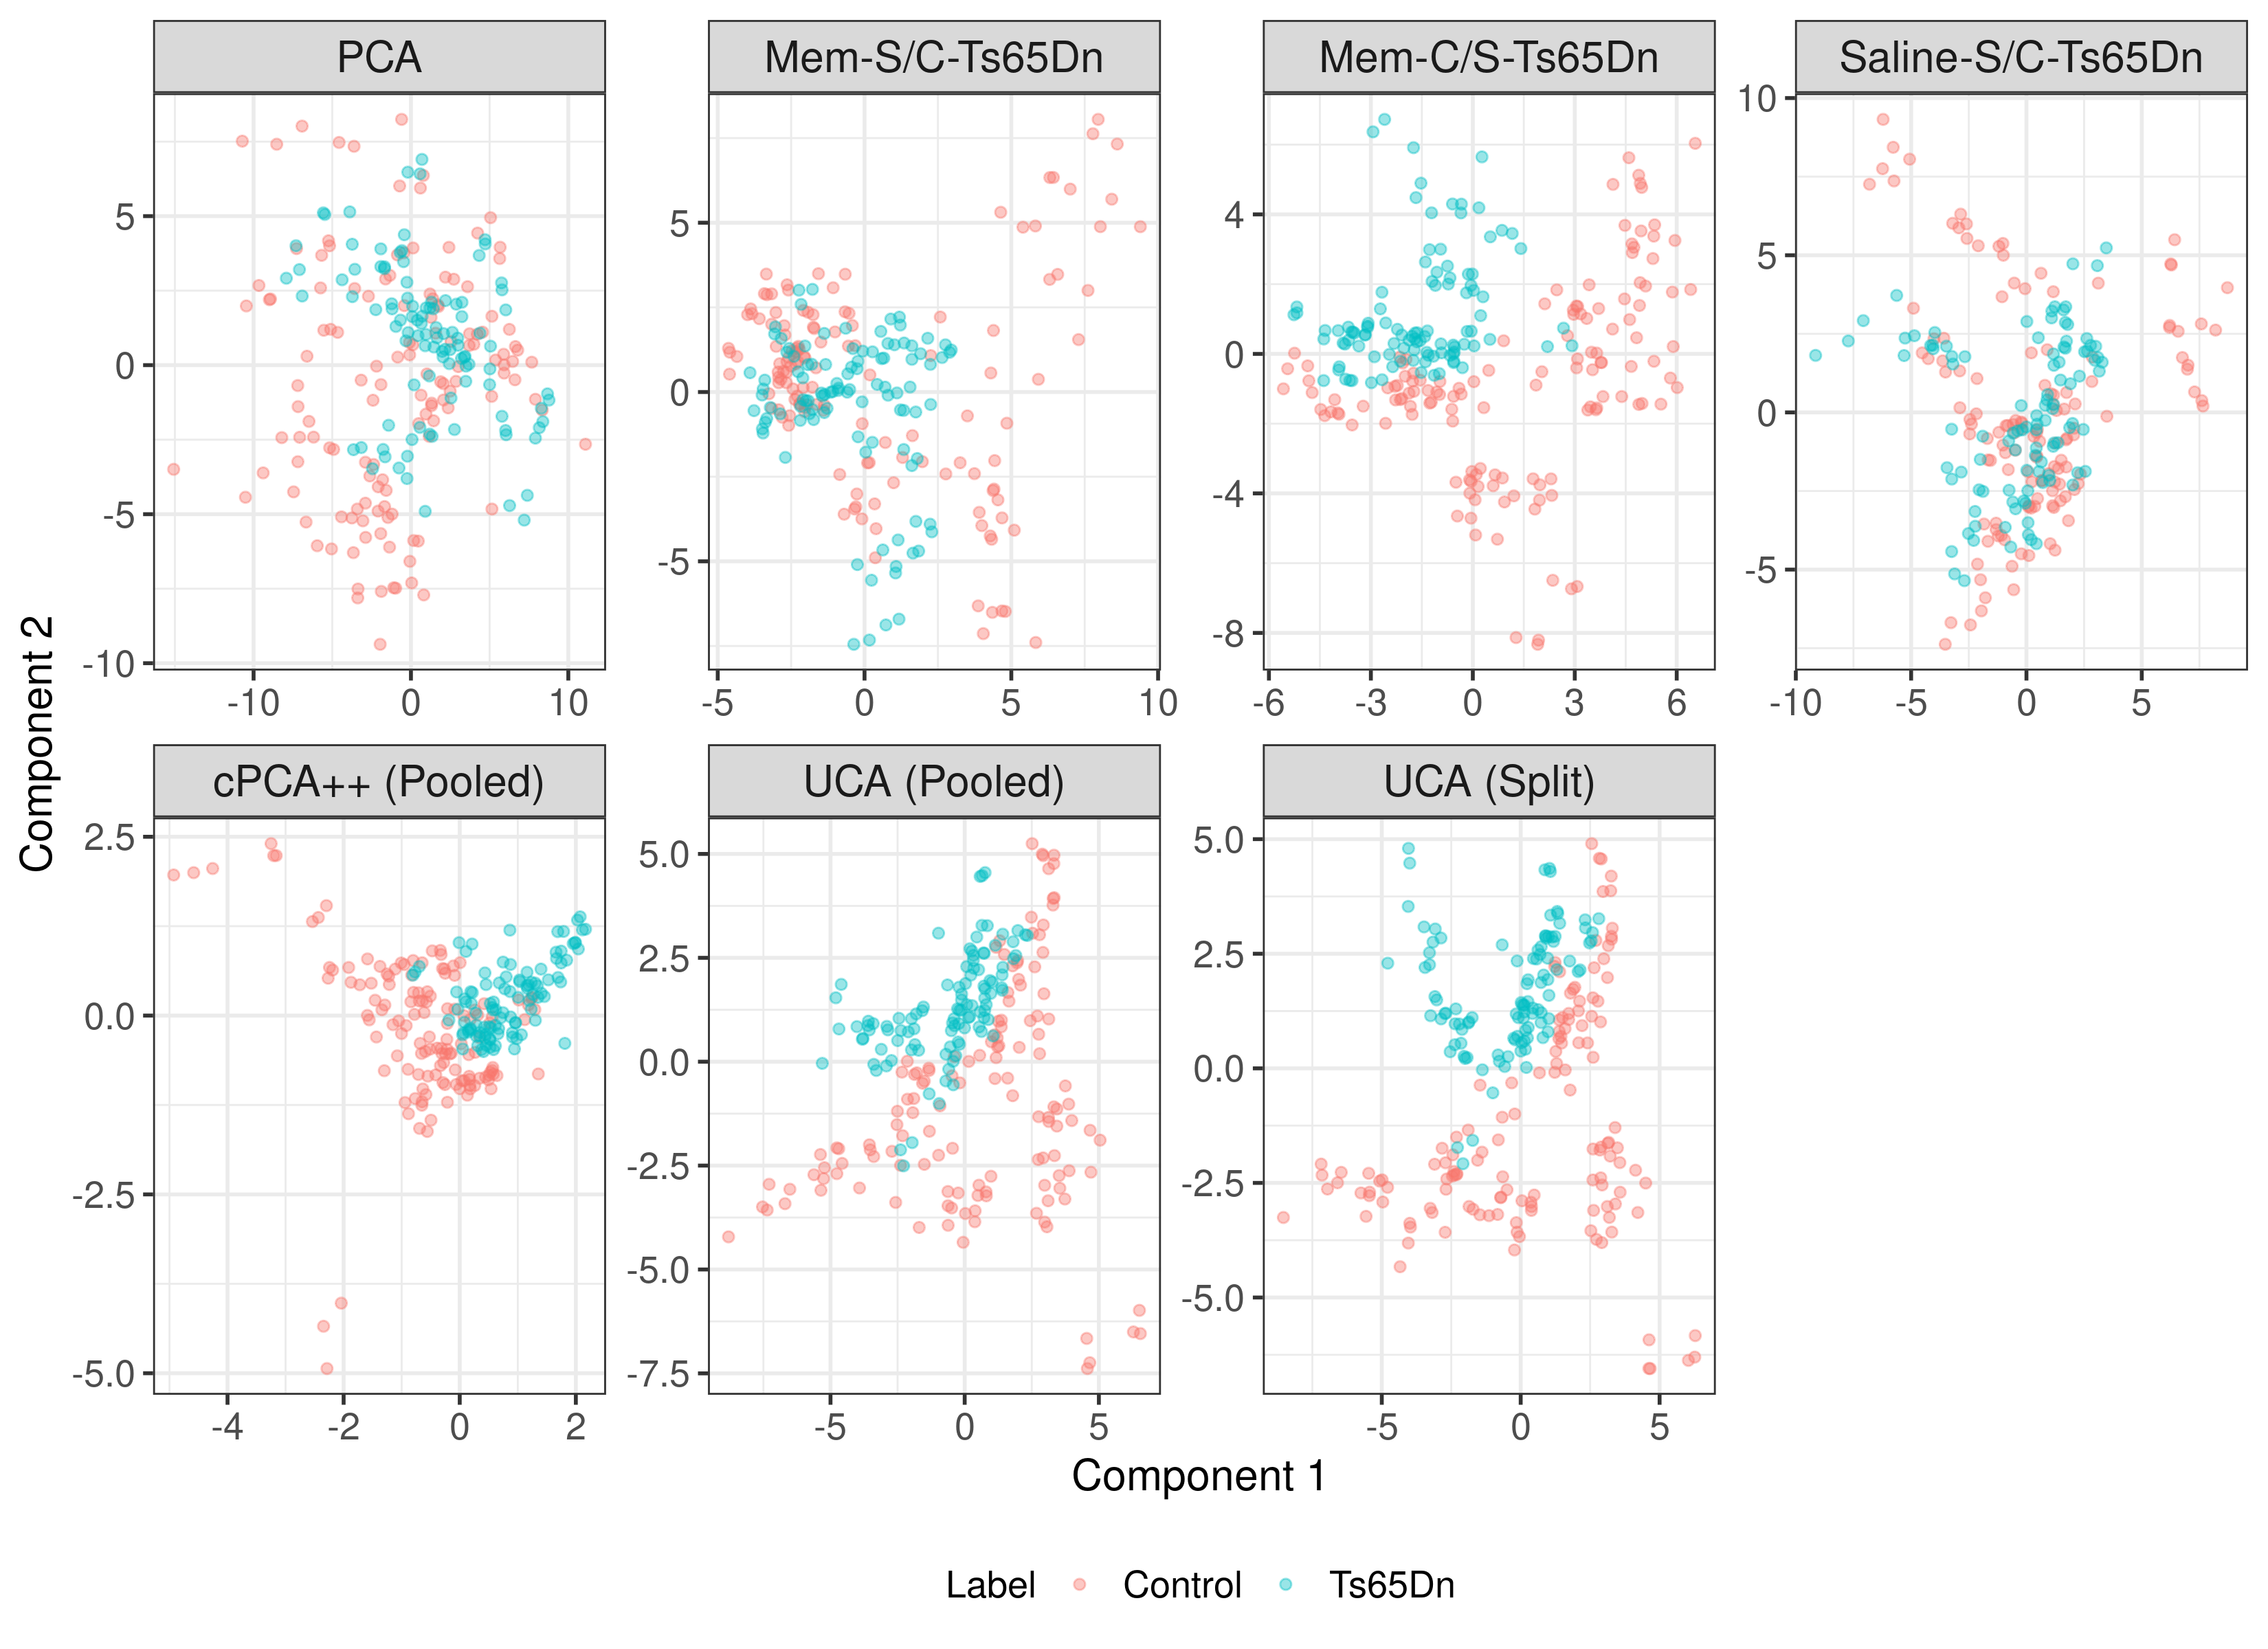
\includegraphics[width = 1.0\textwidth]{figure/Mouse_split_stack_Ts65Dn.png}
	\caption{Mouse Protein Expression : Separability of saline injected mice which were shocked. Separating Down Syndrome and control mice is more difficult in this case when only using a single background dataset. UCA with every combination of background (in parenthesis) represents the best case sceario for cPCA, and cannot separate between Down Syndrome and control mice. However, when combining information from all backgrounds via stacking, UCA improves the separation. Note that cPCA++ and rPCA both have difficulty even when leveraging the same stacked background.  When treating each background separately, UCA improves on the stacking results.}
	    \label{fig:MouseSplitStack}
\end{figure}


%We show that our results match the cPCA results
%We show that cPCA depends on tuning parameter
%results of cPCA++ aren't impressive
%residual PCA yields similar results.


\subsection{Faces}
We exemplify the advantages of the multiple background capabilities of UCA using the Karolinska Directed Emotional Faces (KDEF) \cite{Calvo2008}, which captured images of 7 emotions, 5 different perspectives, from 70 amateur actors in either a practice or final session.
Here we construct an example demonstrating that using UCA with multiple backgrounds is superior to using a single background. 
This is similar to a real world use-case of UCA where researchers may have targeted variation of interest, but also various control groups.
For illustrative purposes, We focus on  uncover variation unique to the Disgust emotion after contaminating the data with Surprise and Angry emotions from the final session.
In Figure \ref{fig:Faces}, we look at the top five eigenfaces produced by PCA, UCA with a single practice session background emotion of either Angry, Surprise, or an amalgamation of both Angry and Suprise (Stack), compared to cPCA++ with stacked background and UCA with dual practice session backgrounds of Angry and Suprised (Split). 
% Since UCA represents the best case, we did not compare to different values of contrastive tuning parameter alpha

% some conclusions about the image

With PCA, eigenfaces represent faces that appear mostly angry.  
UCA with only Surprise practice faces as the background is dominated by surprise faces.
UCA with only Angry practice faces as the background contains a mixture of surprise (2) and disgust (1,4,5) faces.
When UCA has both Surprise and Angry in the background, we see that features of digust are highlighted in the first two eigenfaces
However, when using the joint covariance of Surprise and Angry as the background, features of disgust are pushed until the 3rd eigenface. The 2nd eigenface here closely resembles that from the 3rd eigenface of Split, and the third eigenface closely resembles the 2nd eigenface from split.

Using cPCA++ with the stacked background, I'm not sure what we get. it looks pretty bad.


To better see the differences between the eigenfaces, we project the faces onto the first two components found and color the points by emotional class in figure \ref{fig:Face_Projections}.

\begin{figure}[!th]
    \centering
	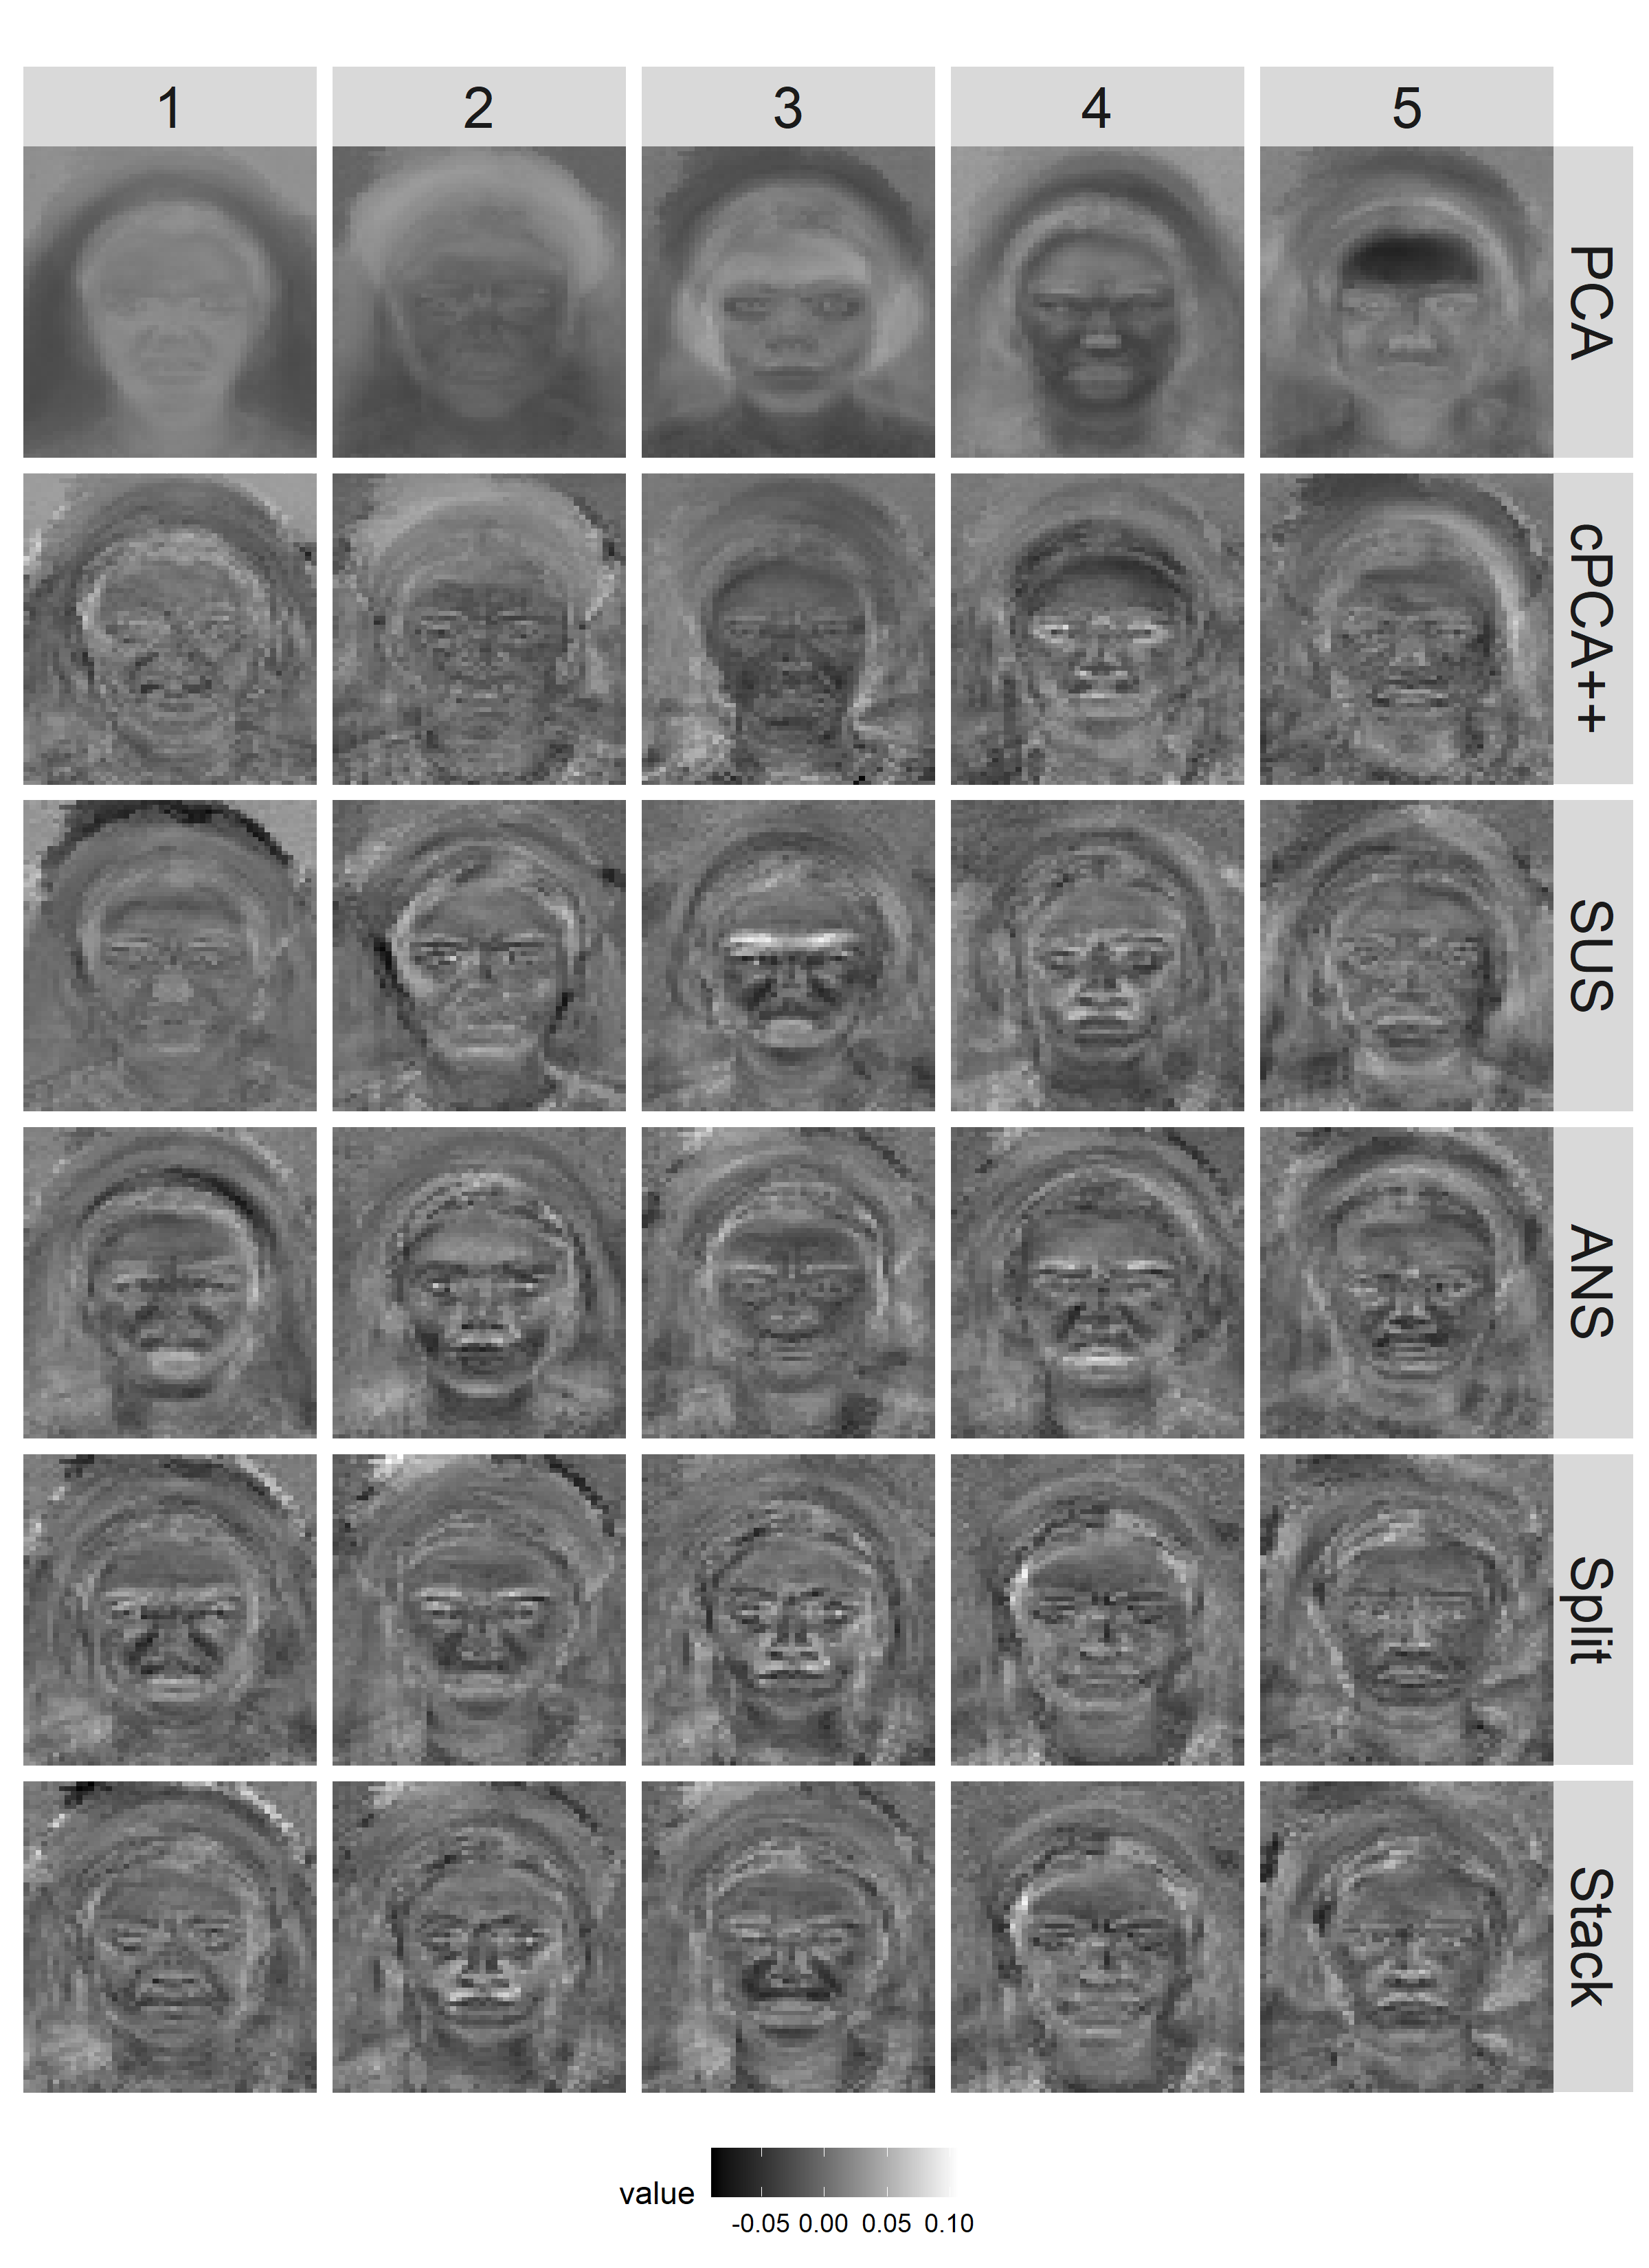
\includegraphics[width = 0.93\textwidth]{figure/F_Surprise_Angry_Disgust.png}
	\caption{First Five Eigenfaces of Surprise, Angry, and Disgust emotions from the Female Actors from Karolinska Directed Emotional Faces (KDEF) \cite{Calvo2008}. Target data is sus/ans/dis }
	    \label{fig:Faces}
\end{figure}
\begin{figure}[!th]
    \centering
	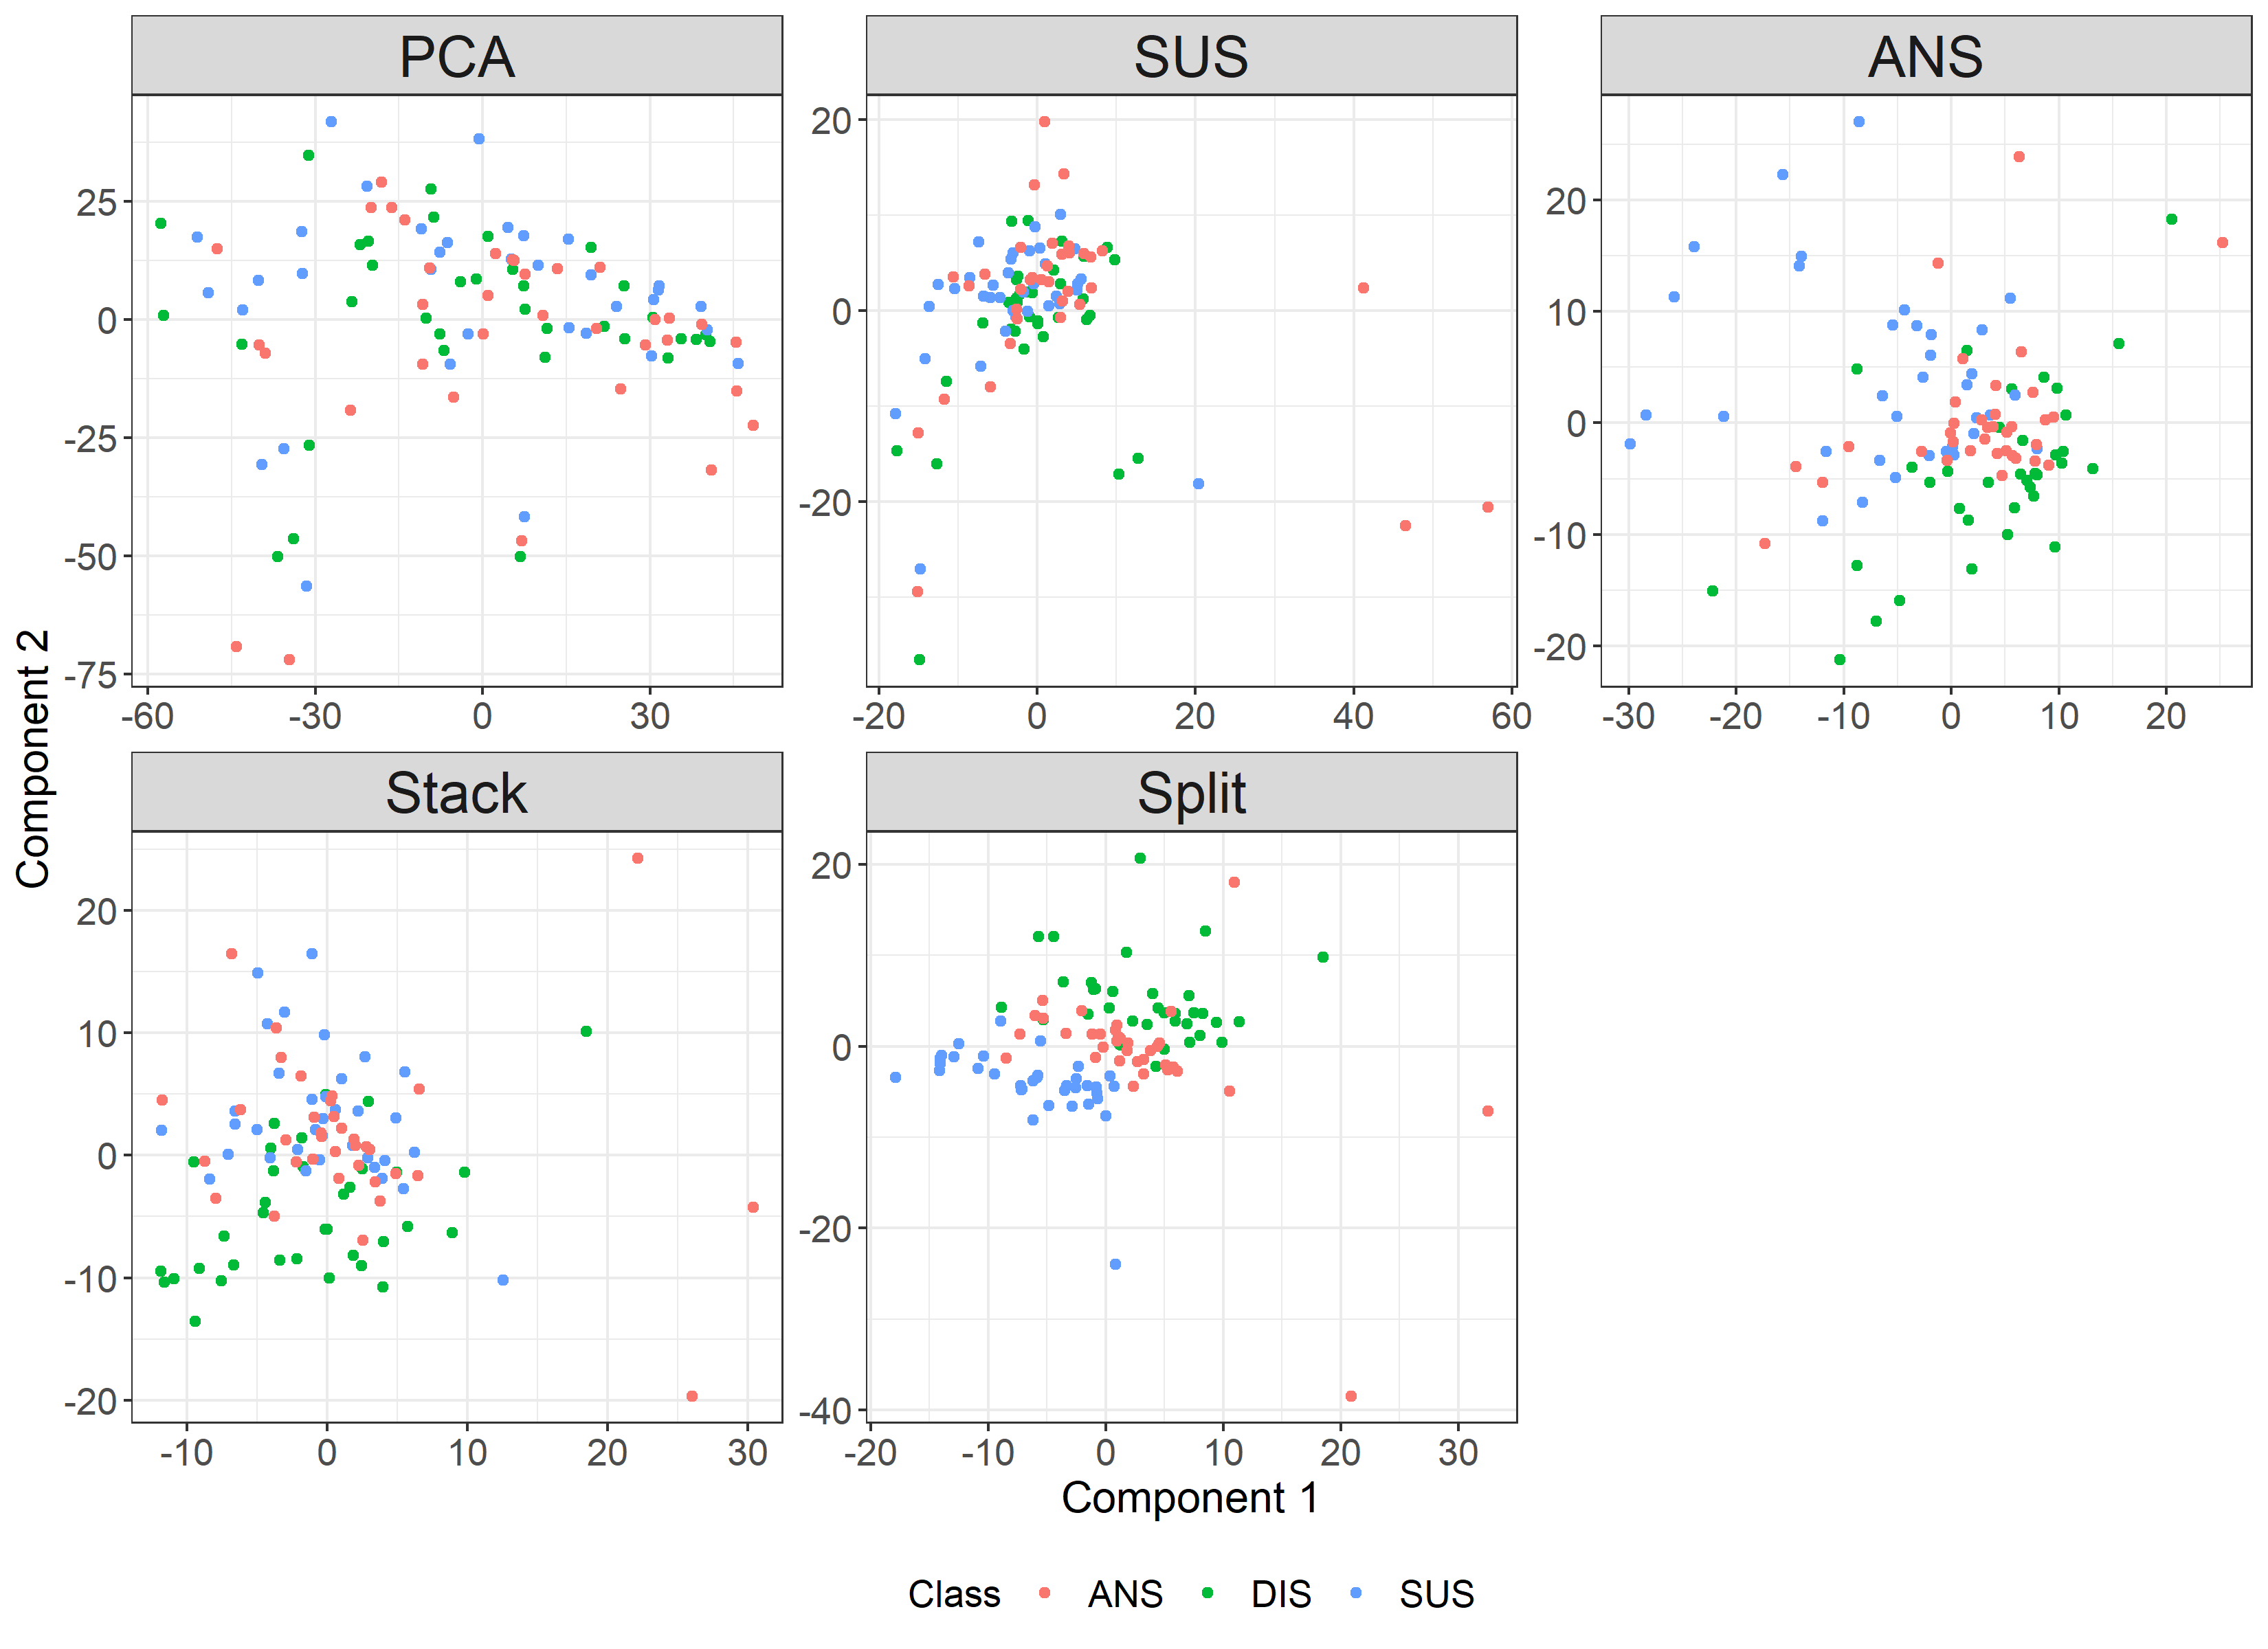
\includegraphics[width = 0.93\textwidth]{figure/F_Surprise_Angry_Disgust_projected.png}
	\caption{Eigenfaces projected onto the first two components found by PCA, cPCA++, UCA using Surprise (SUS) as the background, UCA using Angry (ANS) faces as the background, UCA using both Surprise and Angry as the background treated separately (Split), UCA using the joint covariance of Surprise and Split (Stack) as the background}
	\label{fig:Face_Projections}
\end{figure}

%\begin{figure}[!ht]
%    \label{fig:Diff_faces}
%    \centering
%	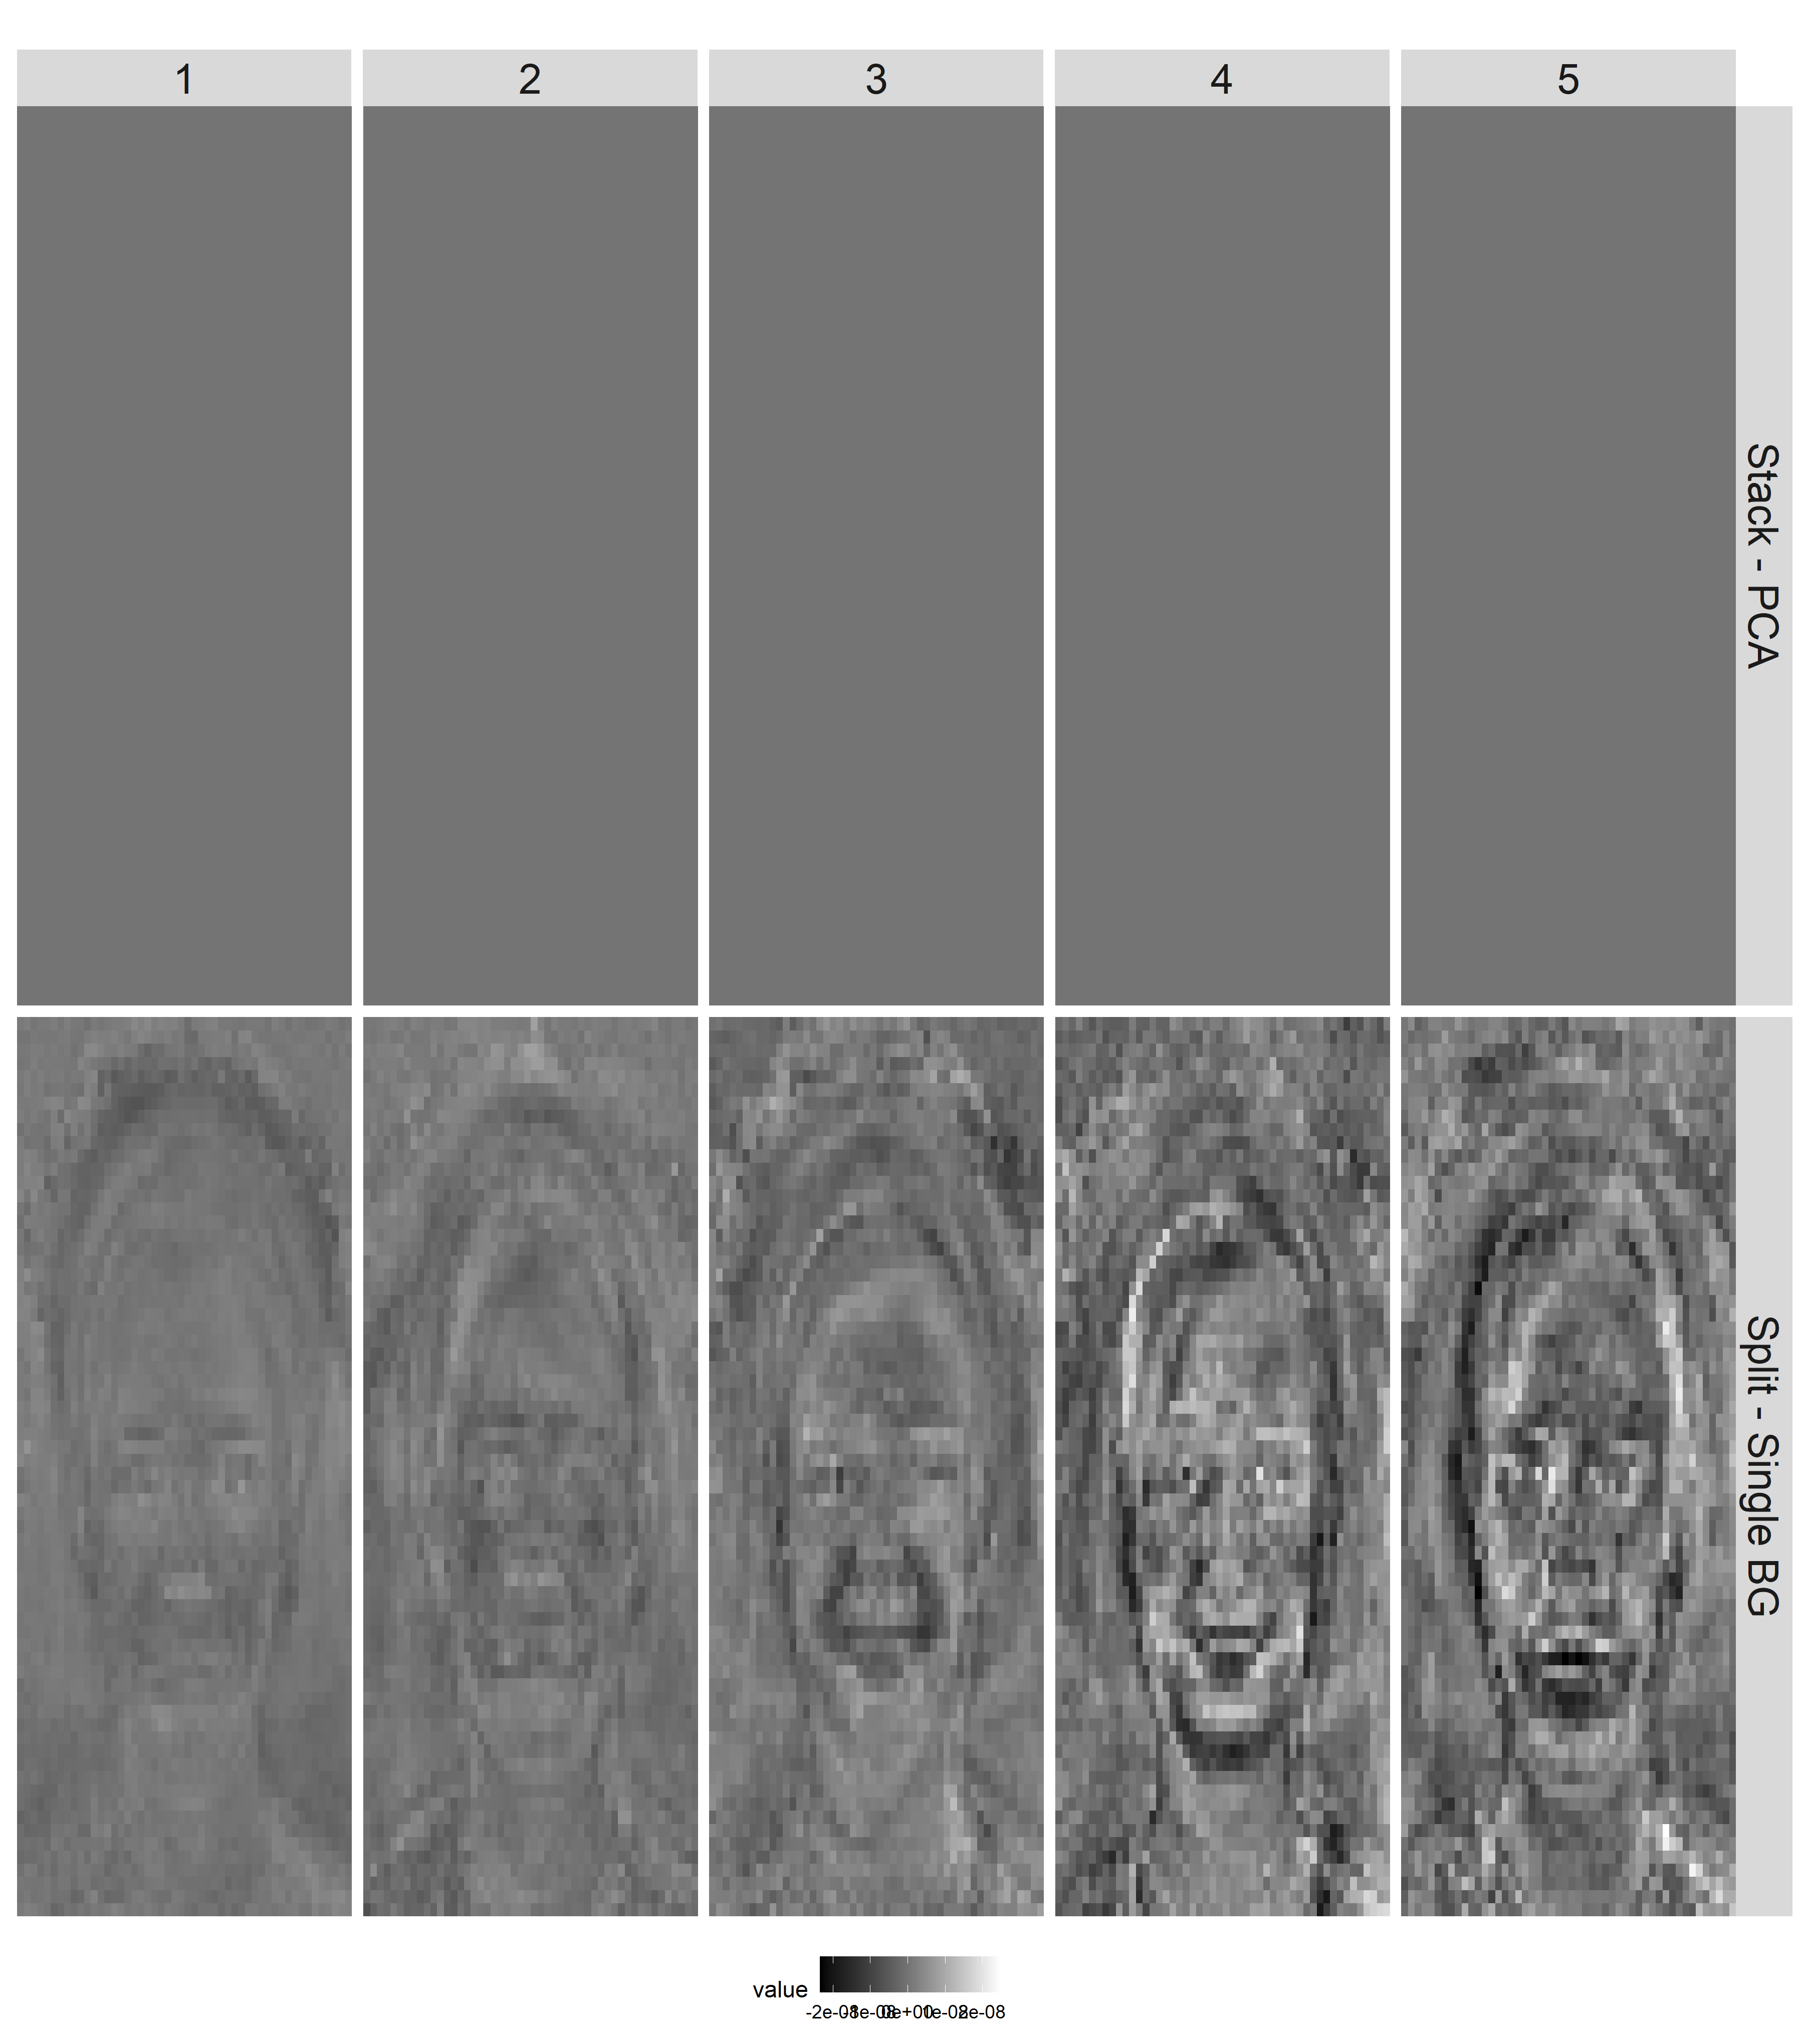
\includegraphics[width = 0.8\textwidth,height = 9cm]{figure/Happy_Neutral_Diff.png}
%	\caption{Eigenface difference images. Top row shows the difference between the eigenfaces produced by using a background of stacking neutral and neutral-inverse practice images, and PCA (no background image). The difference demonstrates that stacking multiple background data sets may lead to background data that is uninformative relative to the target, leading to features no different than PCA.  In contrast, when using UCA with two backgrounds where one background is uninformative (neutral practice and neutral-inverse faces as background), we get similar results to the single background (using only neutral practice faces) results}
%\end{figure}


%\subsection{MNIST}
%We use the numerical image data from MNIST \cite{MNIST} data to further illustrate the advantages of using multiple backgrounds as compared to a single background. This data contains 60,000 labeled training points and 10,000 labeled testing points of digits '0' through '9'.  In this example, we focus specifically on the numbers '4' and '9', which are among the most frequently confused numerical pairs.
%We compared PCA and UCA on the testing images of '4' and '9' under 4 scenarios: using only training images of '4', only training images of '9', combining training images of '4' and '9' via stacking, and utilizing training images of '4' and '9' separately (splitting).  This analysis shows us how the testing images of '4' and '9' load on the directions of maximal variation unseen in the background training images.

%The results of the rotated testing points of '4' and '9' using the first two components of PCA and UCA are seen in figure \ref{fig:MNIST}. It is clear that from the first two components, PCA has difficulty discerning differences between '4' and '9'. When using either '4' or '9' from the training data, the respective variability in the testing data is reduced. To reduce variability of both '4' and '9' in the testing data using the cPCA framework, we stack both the '4' and '9' training data together. However, after stacking, the rotated testing data of '4' and '9' overlap much more significantly than using either one individually, likely due to signal washout when constructing the joint background covariance matrix.  This effect is largely avoided when we treat '4' and '9' separate and construct separate covariance matrices with the training images: the testing points are more separable than using only the '4' background training data, only the '9' background training data, and stacking the '4' and '9' training data to construct a joint training covariance matrix.


%\begin{figure}[H]
%    \label{fig:MNIST}
%    \centering
%	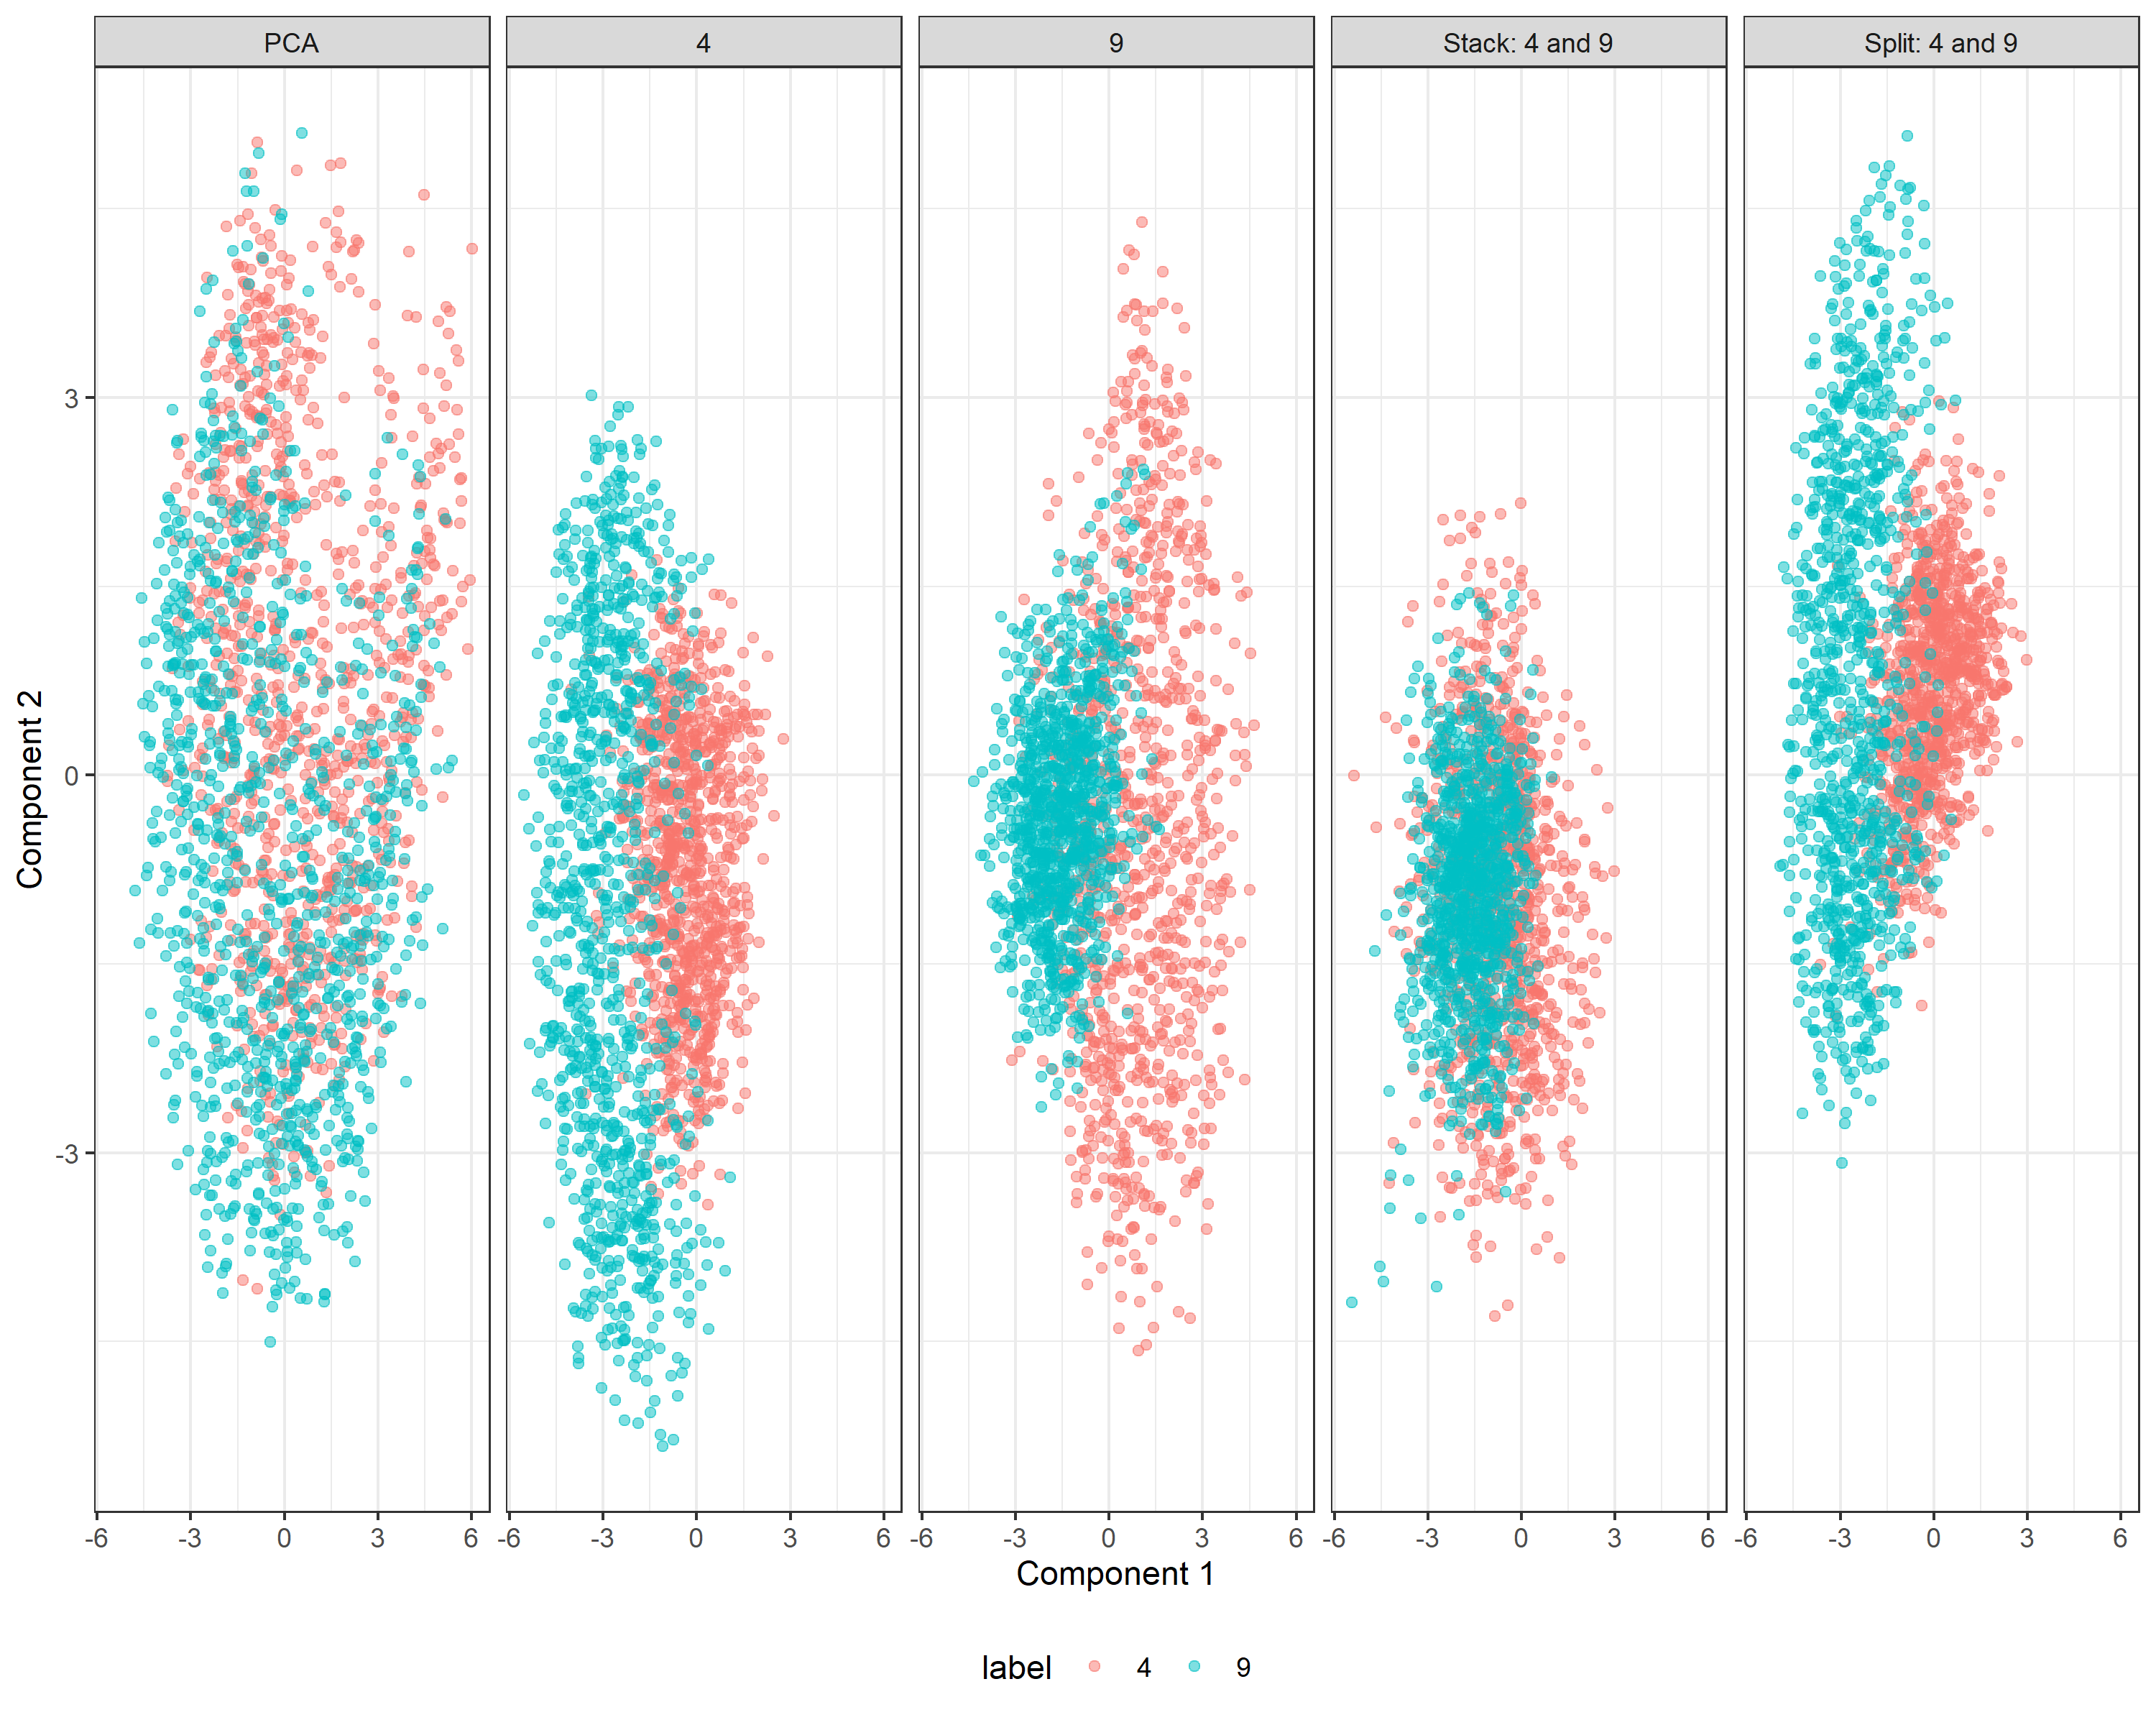
\includegraphics[width = 1.1\textwidth]{figure/MNIST_4_9_Stack_Split.png}
%	\caption{MNIST Data  \cite{MNIST} on the numbers '4' and '9', two commonly confused numerical values.  The target data consists of '4' and '9' from the testing portion of the MNIST data.  The background data (panel label in parenthesis) consists of nothing (PCA), only the labels '4' (4), only the labels '9' (9), both the labels '4' and '9' stacked as if it came from the same label group (Stack: 4 and 9), and the labels '4' and '9' if they were treated as separate backgrounds (Split: 4 and 9).  
%    The numbers '4' and '9' are not easily separable using PCA. Better separability is achieved when either '4' or '9' training data is used in the background.  }	
%\end{figure}

\section{Discussion}
In many data analytics settings we are interested in removing uninteresting variation that contaminate the data of interest
We propose an update to the original cPCA framework, UCA, by extending contrastive abilities to multiple background data. To do this, we first solved the tuning parameter problem which plague current methods. UCA does not require user input in selecting the best contrastive parameter, rather it works by maximizing the target data variability subject to keeping the variability in each background small using weak duality of Lagrangians. Furthermore, we reformulate the contrastive problem to avoid creating several $p \times p$ covariance matrices, enabling us to perform contrastive analysis in high-dimensions.

We show that UCA performs adequately as compared to cPCA, cPCA++, and rPCA in the easily separable case within the mouse data. We then presented a less separable case with the mouse data, in which cPCA, cPCA++, and rPCA fail to do an adequate job in separating Down Syndrome and control mice.  We then showed how leveraging multiple backgrounds allows us to better separate Down Syndrome and control mice than each individual background dataset and simply stacking the individual datasets together. Lastly, we demonstrate how UCA can be used at highlighting emotions in eigenfaces and show that we can construct an example where stacking individual background data can cause cPCA to fail.


%cPCA++ isn't all that impressive
% background data choice is still very important. mouse data with control background gave terrible results

\section{Method}
In this section we introduce Unique Component Analysis (UCA) and show how we arrive at an optimal solution to the contrastive problem. Next, we will extend UCA
to incorporate multiple background data sets. Finally, we address the high-dimensional limitation of cPCA and related methods in both single and multi-background scenarios using the Product SVD method to find our largest eigenvalue and corresponding eigenvector.  

Let background data $X_{n_{x}\times p}$ and target data $Y_{n_{y} \times p}$ be two data sets of sample size $n_x$ and $n_y$ where $X, Y \in \mathbb{R}^{p}$ with respective $p \times p$ dimensional emperical background covariance matrix $B$ and target covariance matrix $A$.
The goal of cPCA is to find the directions of variability, $v \in \mathbb{R}^p$, which account for large variation in the target data $Y$ and small variation in the background data $X$ where $\|v\|_2 = 1$. 
Similar to PCA, cPCA measures variation along direction in target and background matrix with $v^T A v$ and $v^T Bv$ respectively.
For some tuning parameter $\lambda \in \mathbb{R}$, these directions can be isolated by identifying the eigenvector $v$ such that:
\[\text{arg}\max_{v \in \mathbb{R}^p}{\left(v^TAv - \lambda v^TBv\right)} = \text{arg}\max_{v \in \mathbb{R}^p}{v^T\left(A - \lambda B\right)v}\]
For a given $\lambda$, the direction is simply the eigenvector of the weighted difference between covariance matrices where $v$ maximize the variation in $A$ while constraining variation in $B$. 
The tuning parameter $\lambda$ represents how strongly background variation is minimized. When $\lambda = 0$, background variation isn't accounted for, thus the cPCA is reduced to PCA. But as $\lambda$ increases, the relative background variation becomes more dominant, resulting in $v_\lambda$ to focus on directions which minimize background variation rather than maximizing the target. For very large values of $\lambda$, $v_\lambda$ finds the directions which map to the null space of the background data, which effectively is PCA of the target data after being projected onto the orthogonal complement of the background.  Thus, the choice of $\lambda$ can heavily influence the resulting eigenvector. Currently there are no rigorous ways in the choice of $\lambda$.

\subsection{Unique Component Analysis: Single Background}
 We introduce the Unique Component Analysis (UCA) framework to identify the optimal contrastive parameter, $\lambda$, and the resulting directions of variation using the duality of lagrangians.
 By adding the additional constraints of $v^T v = 1$ and $v^T Bv = 1$ we arrive at an objective method to choose $\lambda$. Specifically the primal optimization problem UCA solves is:
     \begin{align}
         &\max_{v\in \mathbb{R}^p}{v^TAv} \label{eq:1} \\ \text{subject to }&\; v^{T}v=I,\;\; v^TBv \leq 1 \nonumber
     \end{align}
    We can solve \ref{eq:1} using weak duality of Lagrangians, $\mathcal{L}$ :
     \begin{align}
         \max_{\lambda \geq 0}{\max_{v\in \mathbb{R}^{P}}{\mathcal{L}}}\left(v,\lambda\right) &= \max_{\lambda \geq 0}{\max_{v\in \mathbb{R}^{P}}{\left( v^TAv - \lambda\left(v^TBv - 1\right)\right)}} \nonumber\\
         &= \max_{\lambda \geq 0}{\max_{v\in \mathbb{R}^{P}}{\left(v^T\left(A - \lambda B\right)v + \lambda\right)}}\nonumber\\
         &= \max_{\lambda \geq 0}{\left(\lambda_{\text{max}}\left(A - \lambda B\right) + \lambda\right)} \label{eq:2}
     \end{align}
     
    where $\lambda$ is the Lagrange multiplier associated with the constraint $v^TBv \leq 1$ and $\lambda_{max}\left(\cdot\right)$ is the largest eigenvalue associated with $A - \lambda B$. Although we have two constraints, we get $v^T v = I$ through Eigen decomposition. This is slightly different from cPCA++, where $v^{T}v$ is not necessarily orthonormal. 
    
    To solve for the largest Lagrange Multiplier, $\lambda$ we follow the standard method of taking the derivative of the Lagrangian $\mathcal{L}$ with respect to the Lagrange Multiplier $\lambda$ and set the derivative equal to zero: 
    
    \begin{align}
   \frac{\partial}{\partial\lambda} \max_{v\in \mathbb{R}^{P}}\mathcal{L}\left(v,\lambda\right) &= \frac{\partial}{\partial\lambda}\left(\lambda_{max}\left(A-\lambda B\right)  + \lambda\right) \nonumber \\ 
   &= 1-v_{\lambda}^{T}B v_{\lambda} = 0 \label{eq:3}
    \end{align}
    
    where $v_\lambda$ is the eigenvector associated with the largest eigenvalue for particular $\lambda$.
    
\begin{algorithm}[ht]
\label{alg:uca-single}
\caption{UCA Single Background}
\SetAlgoLined
  \textbf{Input:} centered target and background data $X$ and $Y$, initial $\lambda$, and the number of components $k$ \; 
  Compute the emperical covariance matrices:
  \[A = \frac{1}{n_y}Y^TY,\;\; B = \frac{1}{n_x}X^TX \] \; Calculate  $C_\lambda = A - \lambda B$ \;
  Find $v_\lambda$ by performing eigen decomposition on $C_\lambda$\;
  \While{$1 - v_{\lambda}^TBv_{\lambda}\neq 0$ }{
    Update $\lambda\leftarrow \lambda + \text{something}$  \;
    Calculate $C_\lambda = A - \lambda B$\; 
    Find $v_\lambda$ by performing eigenvalue decomposition on $C_\lambda$
  }
  compute $V_k\in \mathbb{R}^k$, spanned by the top $k$ eigenvectors of $C_\lambda$\;
  \textbf{Return:} $V_k$ \;
\end{algorithm}
    We use an iterative algorithm (L-BFGS-B) \cite{byrd1995limited} to optimize between finding the Lagrange Multiplier $\lambda$, and finding the associated eigenvectors $v_\lambda$, stopping when equation \ref{eq:3} is satisfied.
%     dual problem:
%    \[\min_{\lambda}\{\max_{v}{v_{\lambda}^{T}\left(A - \lambda B\right)v_{\lambda}}+\lambda\}\]
%     this is equivalent to:
%    \[\min_{\lambda}\{\lambda_{max}\left(A - \lambda B\right)+\lambda\}\]
%     first solve for the Lagrange Multiplier via L-BFGS-B which corresponds to eigenvectors that satisfy:
     

 With the optimal Lagrange Multiplier, eigenvector $v_\lambda$ maximizes equation \ref{eq:1}.
Our constraints allows for a natural way to pick the contrastive parameter $\lambda$ in cPCA. Similar to the constrastive parameter, the Lagrange Multiplier can't be less than zero, and allows us to use box constrained optimization methods. 

% comment on uniquness or is this obvious?

%% is it worth mentioning if A, B are the same, lambda = 1? connections to likelihood ratio test?
%% For the special case when covariance matrices $A$ and $B$ are the same, the constraint forces $\lambda = 1$ because as $\lambda \rightarrow 1^-$, the largest eigenvalue approaches zero and for $\lambda \geq 1$, the largest eigenvalue is zero.




\subsection{Unique Component Analysis: Multiple Backgrounds}
Similarly, for multiple backgrounds, again let the $A$ be the target $p \times p$ covariance matrix and $ B_1, \ldots, B_m$ be the $m$ background $p \times p$ covariance matrices constructed from a $n_y \times p$ dimensional Y data matrix and corresponding $(n_{x_1} \times p), \ldots, (n_{x_m}\times p)$ dimensional $X_1, \ldots, X_m$ background data matrices.

One way to incorporate $m$ background would be to use the framework in the single background setting and stack multiple background data sets before calculate the background covariance matrix, creating a weighted average of the covariance matrices. This is sub-optimal since the background covariance matrix with the most samples may not accounts for the all the background noise, therefore potentially washing out background noise from the other smaller background data sets. 

A more natural way to incorporate $m$ background data sets in a more generalized framework would be to append the background matrices like so:
\[\max_{v\in \mathbb{R}^p}{v^T\left(A - \sum^{m}_{j=1}{\alpha_jB_j}\right)v}\]

However, a parameter sweep for each $\alpha_j$ corresponding to background data $B_j$ would be computationally expensive.
We can easily extend our single background covariance method to address the $m$ background covariance scenario by adding additional constraints to Lagrangian, enforcing $ v^TB_jv\leq 1$ for each $m$ background covariance matrix. Specifically, the primal problem of our multiple background UCA is:
 \begin{align}
         &\max_{v\in \mathbb{R}^p}{v^TAv} \label{eq:4}\\ 
         \text{subject to }&\; v^{T}v=I,\;\; v^TB_1 v \leq 1, \ldots, v^T B_m v\leq 1 \nonumber
     \end{align}

Again, using weak duality of Lagrangians, our objective function now can be written as:
\begin{align}
    \max_{\lambda_1,\ldots,\lambda_m \geq 0}{\max_{v\in \mathbb{R}^{P}}{\mathcal{L}\left(v, \lambda_1, \ldots, \lambda_m\right)}}%&=\max_{\lambda_1,\ldots,\lambda_m \geq 0}{\max_{v\in \mathbb{R}^{P}}{\left(v^TAv - \lambda_1\left(v^TB_1v - 1\right)-\ldots -\lambda_m\left(v^TB_mv - 1\right)\right)}}\nonumber \\
    &=\max_{\lambda_1,\ldots,\lambda_m \geq 0}{\max_{v\in \mathbb{R}^{P}}{\left(v^T\left(A - \sum^{m}_{j = 1}{\lambda_j B_j}\right)v + \sum^{m}_{j=1}{\lambda_j}\right)}} \label{eq:5}
\end{align}

For background $j \in 1,...,m$, we can solve for the $j$th Lagrange Multiplier in equation \ref{eq:5} similarly by taking the partial derivative and setting to zero:
\begin{align}
    \frac{\partial}{\partial \lambda_j}\max_{v\in \mathbb{R}^{P}}{\mathcal{L}\left(v, \lambda_1, \cdots, \lambda_m\right)}&=\frac{\partial}{\partial \lambda_j}\max_{v\in \mathbb{R}^p}\left(v^T\left(A - \sum^{m}_{j = 1}{\lambda_j B_j}\right)v + \sum^{m}_{j=1}{\lambda_j}\right)\nonumber\\
    &= \frac{\partial}{\partial \lambda_j}\max_{v\in \mathbb{R}^p}\left(v^T\left(A - \lambda_j B_j \right)v+\lambda_j\right)\nonumber \\ 
    &= 1-v_{\lambda_j}^{T}B_j v_{\lambda_j} = 0 \label{eq:6}
\end{align}

To solve this multiple background dataset problem we propose a coordinate descent algorithm that utilizes the single background dataset L-BFGS-B  \cite{byrd1995limited} algorithm above.
Suppose there are $m$ background data sets, we are on the $k^{th}$ iteration. Let $A_{(j)}^*$ be the variation in $A$ after removing Background variation that is not $B_j$:
     \[A_{(j)}^{*} = A - \sum_{ i = 1 }^{j-1}\lambda_{i}^{(k+1)}B_i - \sum_{i =j+1}^{m}\lambda_{i}^{(k)}B_i \] \
to solve for the each of the $m$ Lagrange Multipliers we use Algorithm \ref{alg:uca-multiple}.

% add input and output into algorithm
\begin{algorithm}[ht]
\label{alg:uca-multiple}
\caption{Coordinate Descent Algorithm for UCA with Multiple Background}
\textbf{Inputs: } $m$ Centered Background data $X_1,\cdots, X_m $, Centered Target Data $Y$, $k$ number of components\;
    Initialize $\lambda_{1}^{(0)}, \cdots,\lambda_{m}^{(0)} $, $\epsilon$\;
  Compute the emperical covariance matrices:
  \[A = \frac{1}{n_y}Y^TY,\;\; B_1 = \frac{1}{n_{x_1}}X_1^TX_1,\;\cdots, B_m = \frac{1}{n_{x_m}}X_m^TX_m\; \]
    \While{$l^{(k+1)} - l^{(k)} > \epsilon$}{
     \For{ $j = 1:m$}{
     Let $A$ in Algorithm \ref{alg:uca-single} be $A_{(j)}^{*}$ and $B = B_j$.
     Solve for $\lambda_j^{(k+1)}$ via Algorithm \ref{alg:uca-single}, corresponding to the largest eigenvalue of \[C_{\lambda_j} = A_{(j)}^{*} - \lambda_j^{(k+1)}B_j\] \
     %with corresponding eigenvector, $v_{\lambda_{j}^{(k+1)}}$, satisfying:
    %\[1 -v_{\lambda_{j}^{(k+1)}}^{T} B_j v_{\lambda_{j}^{(k+1)}} = 0\]
     }
     After iterating through $m$ Lagrange Multipliers, calculate value of Lagrangian
     \[l^{(k+1)} = \lambda_{max}\left(A-\sum^{m}_{j=1}\lambda_{j}^{(k+1)}B_j\right)+ \sum^{m}_{j=1}\lambda_{j}^{(k+1)}\]\
    }
  Compute \[C_{\lambda_1, \cdots, \lambda_m} = A - \sum^{m}_{j = 1}{\lambda_j B_j}\]
  Find $V_k\in \mathbb{R}^k$, spanned by the top $k$ eigenvectors of $C_{\lambda_1, \cdots, \lambda_k}$\;
\textbf{Return: } $V_k$
\end{algorithm}


The advantage to the Lagrangian method in the multiple background setting is that rather than constructing an aggregated covariance matrix by stacking data, which arbitrarily weighs covariance matrices by their sample size, our method objectively constructs weights which satisfy the constraint $ v^TB_jv\leq 1$ for each $m$ background covariance matrix. If multiple backgrounds contain the same information, constructing the covariance matrix by stacking data will change the covariance by a factor less than 1, e.g. if two backgrounds, the covariance changes by $\frac{2}{2n - 1}$.  If only one covariance matrix will constrain the Lagrangian, the corresponding Lagrange Multiplier will be non-zero and Lagrange Multipliers corresponding to all other redundant constraints on the Lagrangian are set to zero.  

\subsection{Extension to High Dimensional Data:}
To extend our method to high-dimensional data, we avoid the traditional Eigen decomposition method of finding eigenvalue/eigenvectors of the covariance matrix. Just like how singular-value decomposition (SVD) of the data matrix can be used to find the top eigenvalue/eigenvectors of it's covariance, we introduce the Product SVD method to exploit the structure of how the contrastive covariance matrices are formed and employ SVD of a product of matrices to quickly find our top eigenvalue.  Breaking the problem down in this way considerably speeds up our L-BFGS-B algorithm, and allows us to run UCA even in the high-dimensional setting.

For a single background, let the $p \times p$ covariance matrices $A$ be the target covariance matrix and $B$ be the background covariance matrix. $A$ and $B$ are formed from corresponding centered $n_y \times p$ target data matrix $Y$,   and centered $n_x \times p$ background data matrix $X$.  We can write the difference of the covariance matrices $A - \lambda B$ as a product of a $p \times (n_y + n_x)$ dimensional left matrix , $L$, and a $(n_y + n_x) \times p$ dimensional right matrix, $R$ as seen in equation \ref{eq:7}:
\begin{align}
C_\lambda &= A - \lambda B \nonumber\\
 &=\frac{1}{n_y}Y^TY -\frac{\lambda}{n_x} X^T X\nonumber \\
 &=  \underbrace{\left[ \frac{1}{\sqrt{n_{y}}}Y^T, - \frac{\lambda}{\sqrt{n_{x}}} X^T\right]}_{L}\underbrace{\begin{bmatrix*} \frac{1}{\sqrt{n_{y}}}Y \\ \frac{1}{\sqrt{n_{x}}}X \\ \end{bmatrix*}}_{R} \label{eq:7}
\end{align}
With this formulation, we can follow the steps in Golub et al.  \cite{Golub}, and find the singular values and vectors of $C_\lambda$ using a sequence of SVD and QR decompositions operating on the left and right matrices. Since singular values and eigenvalues coincide in square matrices, we use the singular vectors, $U$, to find the largest eigenvalues by sorting the diagonal of $ULRU^T$.  
We describe the Product SVD Method in algorithm \ref{algo:product-svd}, which can directly replace the eigen decomposition in the single background UCA (Algorithm \ref{alg:uca-single}).

\begin{algorithm}[h]
\label{algo:product-svd}
\caption{Product SVD Method to calculate the largest Eigenvalue of $C_\lambda$}
\SetAlgoLined
\textbf{Input:} Centered background matrix $X$, centered target matrix $Y$, and $\lambda$\;
\nl Construct 
$  L = \left[ \frac{1}{\sqrt{n_{y}}}Y^T, - \frac{\lambda}{\sqrt{n_{x}}} X^T\right],\;
   R = \begin{bmatrix*} \frac{1}{\sqrt{n_{y}}}Y \\ \frac{1}{\sqrt{n_{x}}}X \\ \end{bmatrix*} $\;
\nl  SVD the right matrix, $R = U_R S_R V^T_R$ \;
\nl  QR decompose $LU_R$ into  $Q_{LU_R}R_{LU_R}$ \;
\nl  SVD the product of $R_{LU_R}$ (step 3) and $S_R$ (step 2), $R_{LU_R}S_{R} = EDF^T$ \;
\nl  The singular vectors of $C_\lambda$ is the product of $Q$ (step 3) and $E$ (step 4), $U_{C_\lambda} = Q_{LU_R}E$ \;
\nl  Find the largest eigenvalues of $C_\lambda$ by sorting the diagonal of $D_{C_\lambda}$, where $D_{C_\lambda} = U_{C_\lambda} C_\lambda U_{C_\lambda}^T$ \;
\textbf{Output:} $\lambda_{\text{max}}\left( C_\lambda \right)$ 
\end{algorithm}
 
Similarly, for multiple backgrounds, again let the $A$ be the target $p \times p$ covariance matrix and $ B_1, \cdots, B_m$ be the $m$ background $p \times p$ covariance matrices constructed from a $n_y \times p$ dimensional Y data matrix and corresponding $(n_{x_1} \times p), \cdots, (n_{x_m}\times p)$ dimensional $X_1, \cdots X_m$ background data matrices.

We can construct $C_{\lambda_1, \cdots, \lambda_m} = A - \sum^{m}_{j=1}\lambda_jB_j$ analogously by appending the additional data sets to the left and right matrices:
\begin{align}
C_{\lambda_1, \cdots, \lambda_m}&= A - \sum^{m}_{j=1}\lambda_jB_j \nonumber \\
&=\frac{1}{n_y}Y^{T}Y -\sum_{j=1}^{m}{\frac{\lambda_{j}}{n_{x_j}}X_{j}^TX_{j}} \nonumber\\
     &=  \underbrace{\left[\frac{1}{\sqrt{n_y}}Y^T, -\frac{\lambda_1}{\sqrt{n_{x_{1}}}} X^T_1, \cdots, -\frac{\lambda_m}{\sqrt{n_{x_{m}}}}X^T_m\right]}_{L} \underbrace{\begin{bmatrix} \frac{1}{\sqrt{n_{y}}}Y \\ \frac{1}{\sqrt{n_{x_{1}}}}X_1 \\ \vdots \\ \frac{1}{\sqrt{n_{x_{m}}}}X_m \end{bmatrix}}_{R} \label{eq:8}
\end{align}
Using the Coordinate Descent (algorithm \ref{alg:uca-multiple}) to solve for each $\lambda_j$ prescribed above, we can substitute the Eigen decomposition of the covariance matrix, $C_{\lambda_{j}}$ with the Product SVD method (algorithm \ref{algo:product-svd}) using $L$ and $R$ defined in equation \ref{eq:8}.

 The Product SVD method is advantageous in high-dimensions because it never explicitly operates on the entire $p \times p$ covariance matrix. Not only is our method more memory efficient, scaling with $n\times p$ bytes rather than $p^2$ bytes, but our method is also computationally more efficient at finding the largest eigenvalue/eigenvector as operating SVD and QR decomposition on either the left or right matrices is faster than directly operating Eigen decomposition on the covariance matrix. In the single background scenario,  $\lambda$ only appears in $L$. Thus since, $R$ doesn't change, we can pre-compute the SVD of $R$, and only update $L$ when solving for $\lambda_{\text{max}}$.
Similarly, in the multi-background scenario, rather than modifying $A^*$ in the original Coordinate Descent algorithm, this method allows us to only modify the $j+1$ element of the left data matrix, $L$.
 The SVD of the right matrix, $R$, only needs to be computed once in our coordinate descent. Furthermore, at each step within the coordinate descent only step 3 and 4, the SVD and QR, are computed, and are done on matrices with dimensions much smaller than $p \times p$.
 
To demonstrate the speed improvements of the Product SVD method compared to the current fastest implementations of Eigen decomposition in high-dimensions, we conduct a simulation study with 25 sample $100 \times p$ target and background data matrices generated from a standard Normal distribution with $p$ varying from 1.000 to 10,000 in steps of 1,000. To ensure a fair comparison, we leverage C++ in both implementations using a custom RcppArmadillo \cite{rcpparmadillo} function for the Product SVD method and the RSpectra package (0.16-0) \cite{Rspectra} for the Eigen decomposition method; RSpectra being a package designed for large-scale Eigen decompositions based off the C++ Spectra library. We use the microbenchmark package \cite{microbenchmark} to ensure accurate timings. Our benchmark does not take into account the additional cost of forming the $p\times p$ covariance matrices, which would only exacerbate the difference between the two methods in real world applications.

\begin{figure}[!ht]
    \label{fig:computational_perf}
    \centering
	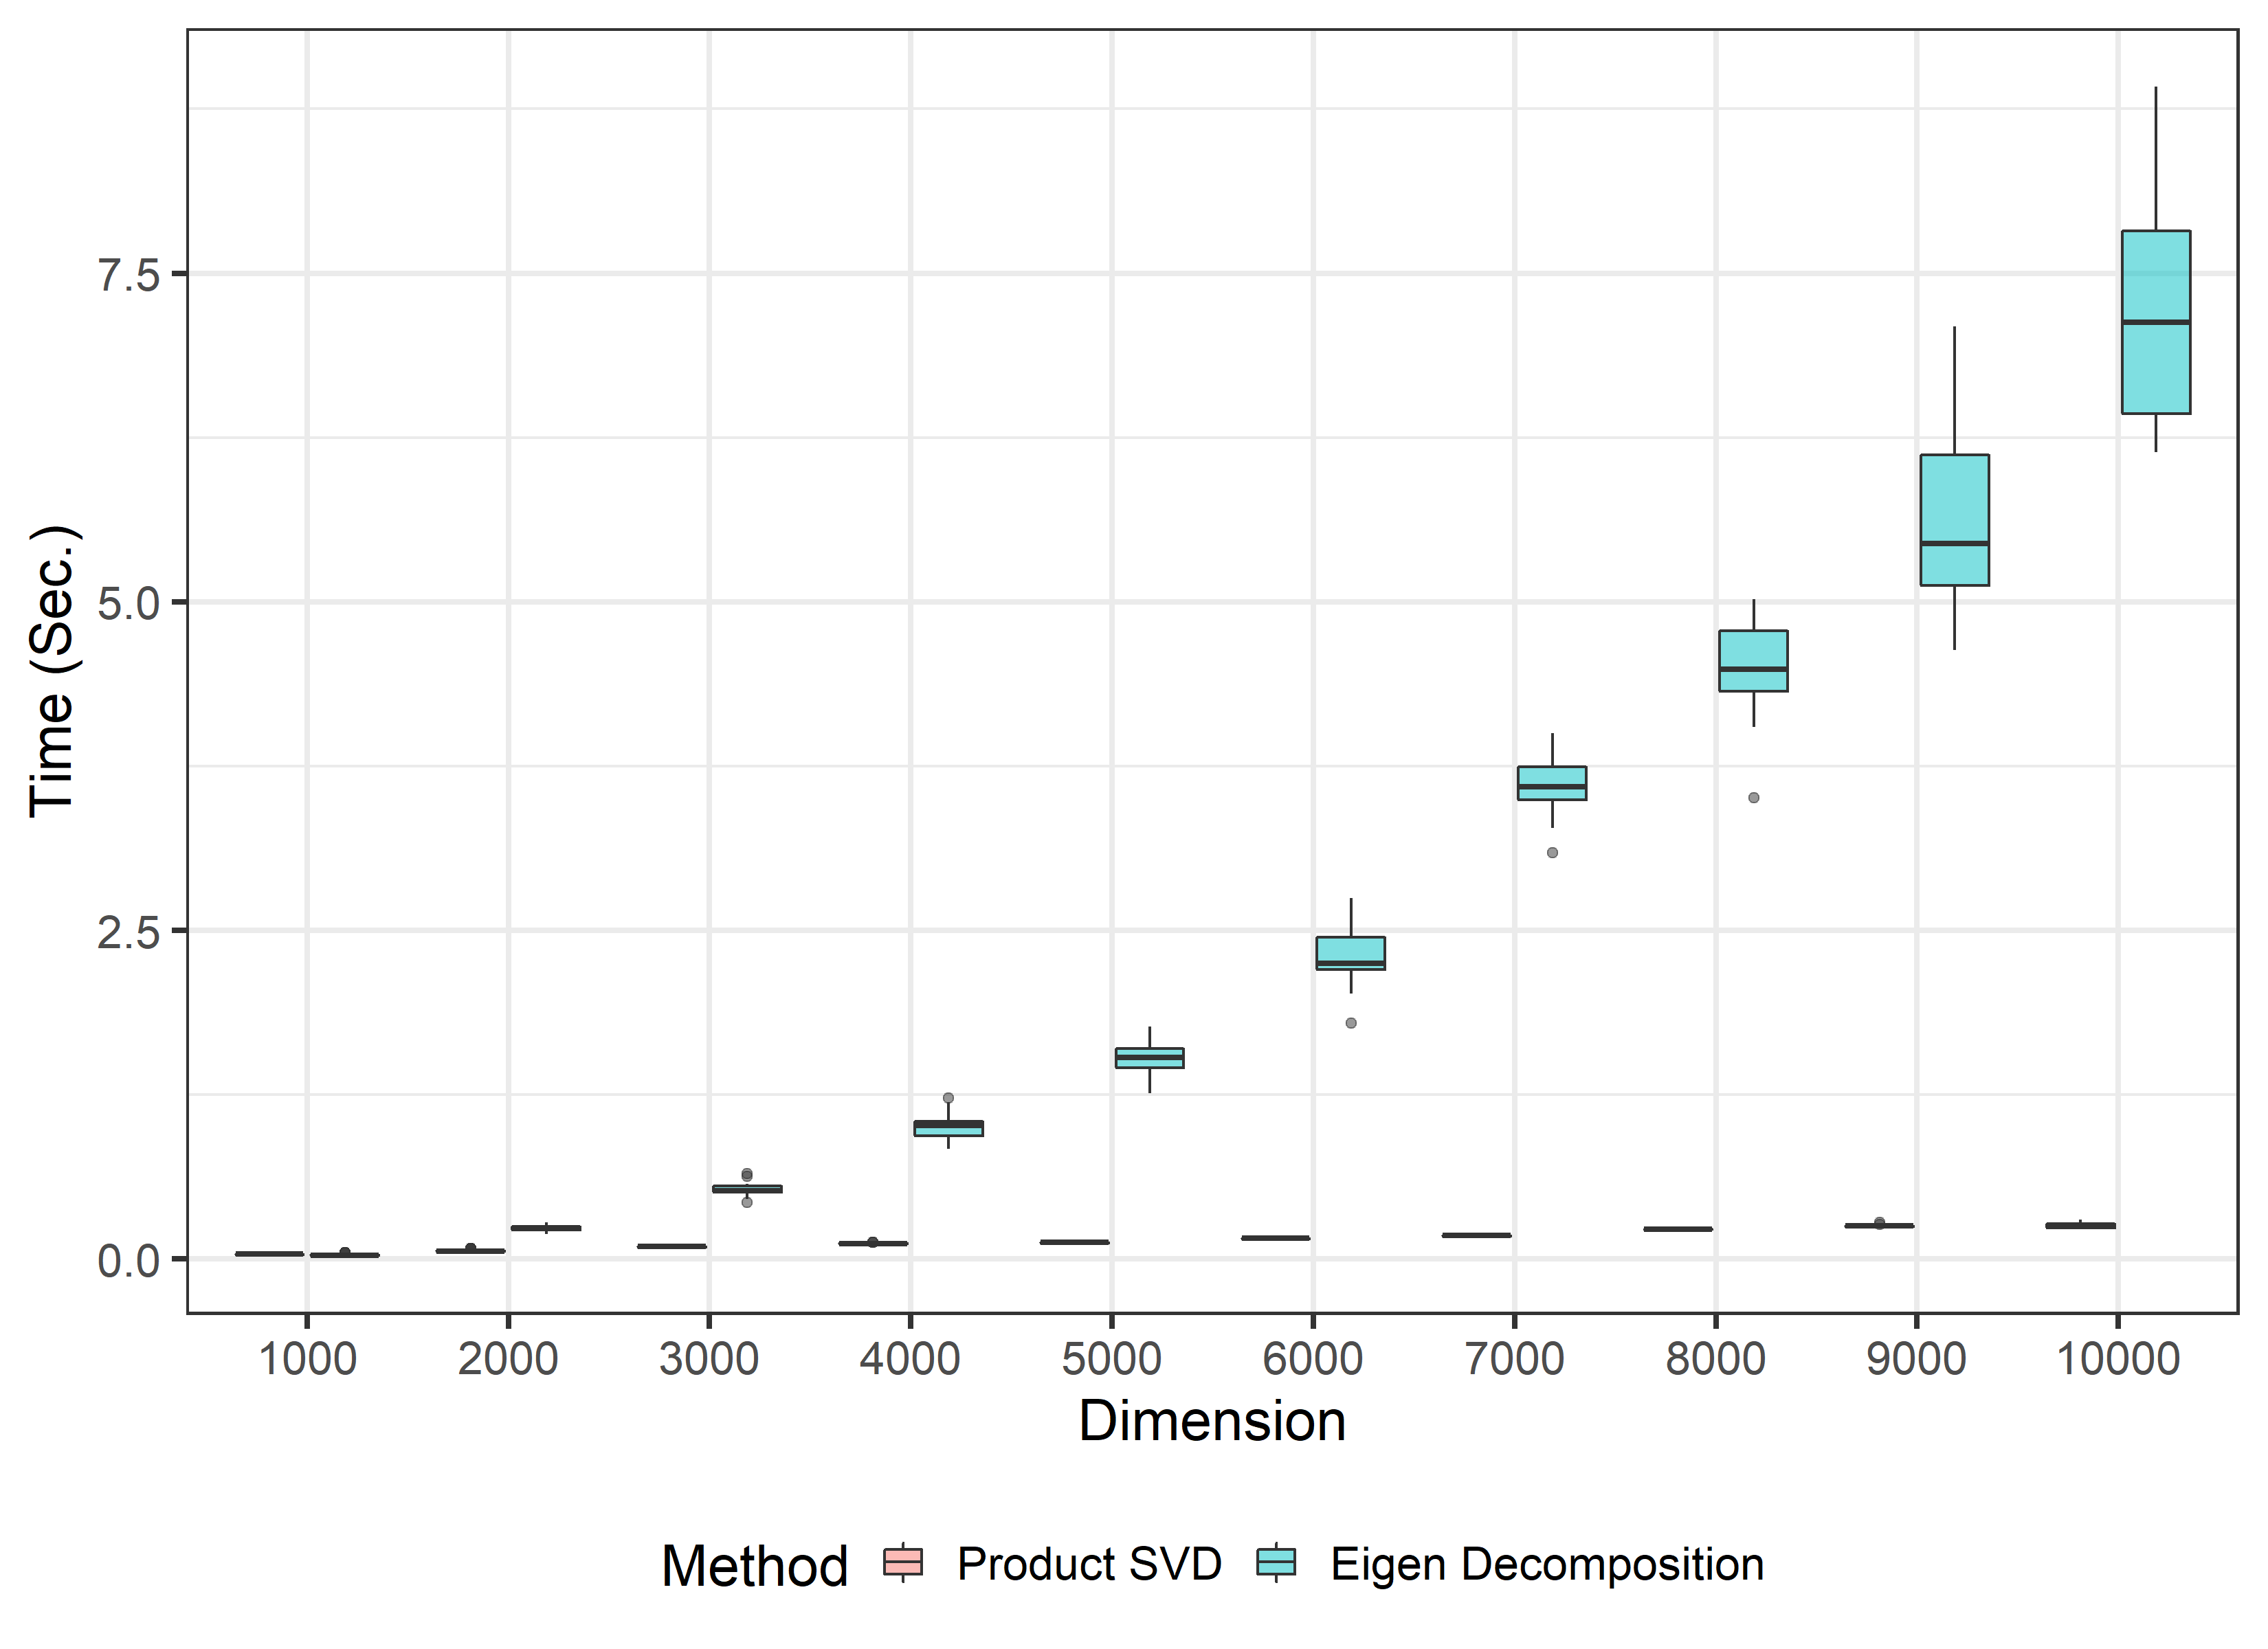
\includegraphics[width = 0.8\textwidth]{figure/final_perf.png}
	\caption{UCA and cPCA implementation using Product SVD vs. Eigen decomposition for high-dimensional data: 25 random $100 \times p $ target and background matrices are generated from a standard normal distribution and where $p$, the dimension varied from 1,000 to 10,000 in steps of 1,000. Box plots of time (in seconds) is plotted for both Eigen decomposition and the product SVD method. For small $p$, there is a negligible difference between the methods. However, as dimension $p$ increases, the Product SVD is significantly faster.}
\end{figure}

Figure \ref{fig:computational_perf} show box plots of time (in seconds) versus the dimension, $p$, colored by method, summarizes the results of the simulation study. As dimension $p$ increases, the computational time of our Product SVD method increases much slower than the current Eigen decomposition implementations. It should be mentioned that for $p < 1000$ the Product SVD method is slower due to overhead of additional computation on small matrices. In general, for low-dimensional settings where $n \geq p$, the Product SVD will be negligibly slower because of the additional QR, SVD, matrix products, and sort computations. 

 %More concretely, an UCA analysis of a target $3400\times 3400$ dimensional covariance matrix with two backgrounds requires 88 MB of storage for each of the three covariance matrices formed, compared to 1.8 MB for each data matrix.  Assuming these matrices have all been pre-calculated, using a RSpectra implementation of eigendecomposition, UCA takes 93 seconds vs. 9 seconds with our method.
 
 All computations in this paper were done with R 3.6.3 \cite{baseR} on an AMD Ryzen 1700X 3.7 gHz processor and 64GB 3000 mhz DDR4 RAM, utilizing the Intel MKL libraries. 
 
 % these subsections are just copies of cPCA paper...
% \subsection{Theoretical Guarantees}
% \subsection{Choosing Background Data}
 \subsection{Code Availability}
 We have released a R implementation of \href{https://github.com/rtud2/Residual-Dimension-Reduction/tree/master/uca}{UCA on GitHub}. We have implemented both Product SVD on the data matrix and Eigen decomposition on the contrastive covariance matrix and allow the background to take either a single background or a list of backgrounds. The GitHub repository also includes R markdown and datasets that reproduce most of the figures in this paper and in the Supplementary.
 
 \subsection{Data availability}
 Datasets that have been used to evaluate UCA in this paper are publicly available from the authors of the original studies. You can download the mouse protein expression dataset from the \href{https://archive.ics.uci.edu/ml/datasets/Mice+Protein+Expression}{UCI Machine Learning Repository} \cite{Higuera} and the Karolinska Directed Emotional Faces (KDEF) from \href{https://kdef.se/}{kdef} website  \cite{Calvo2008}.
 
\newpage
\bibliography{mybib}{}
\bibliographystyle{plain}
\newpage
\section{Appendix}
\begin{figure}[!ht]
    \centering
	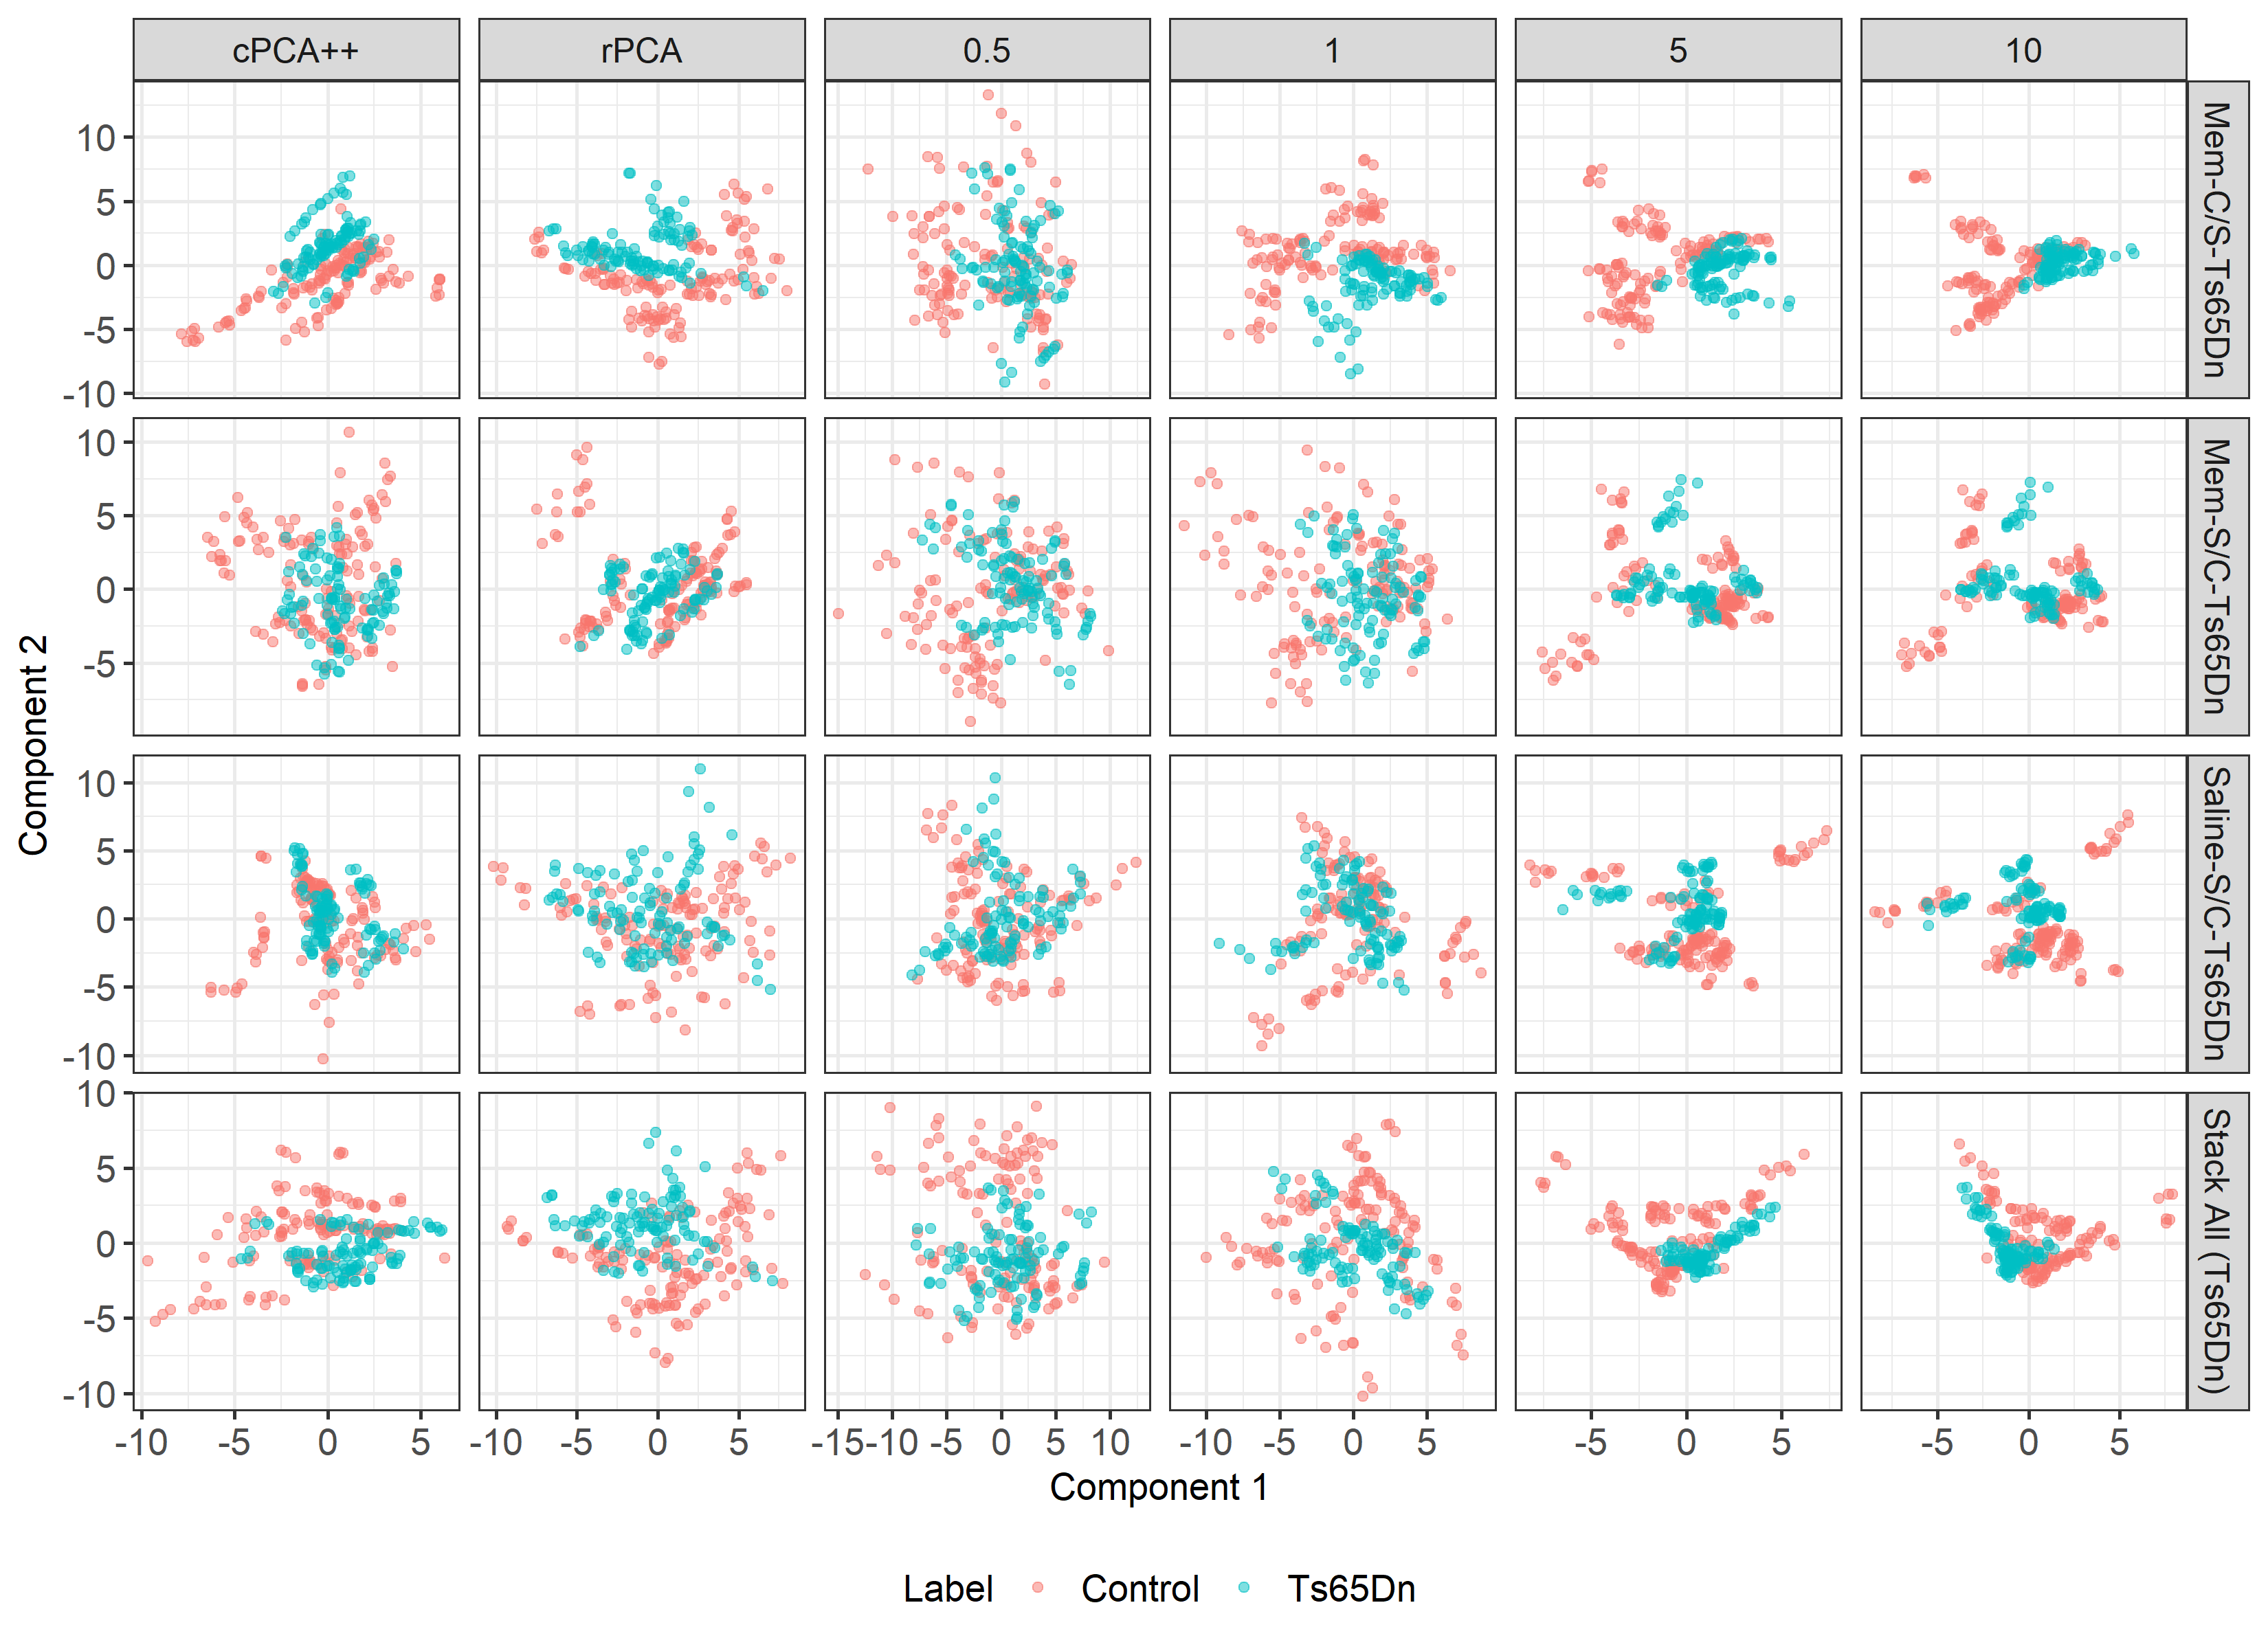
\includegraphics[width = 0.8\textwidth]{figure/Mouse_stack_cpc_rpcTs65Dn.png}
	\caption{Mouse Protein Expression Dataset}
	\label{fig:mouse_stack_cpca}
\end{figure}

\begin{figure}[!ht]
    \centering
	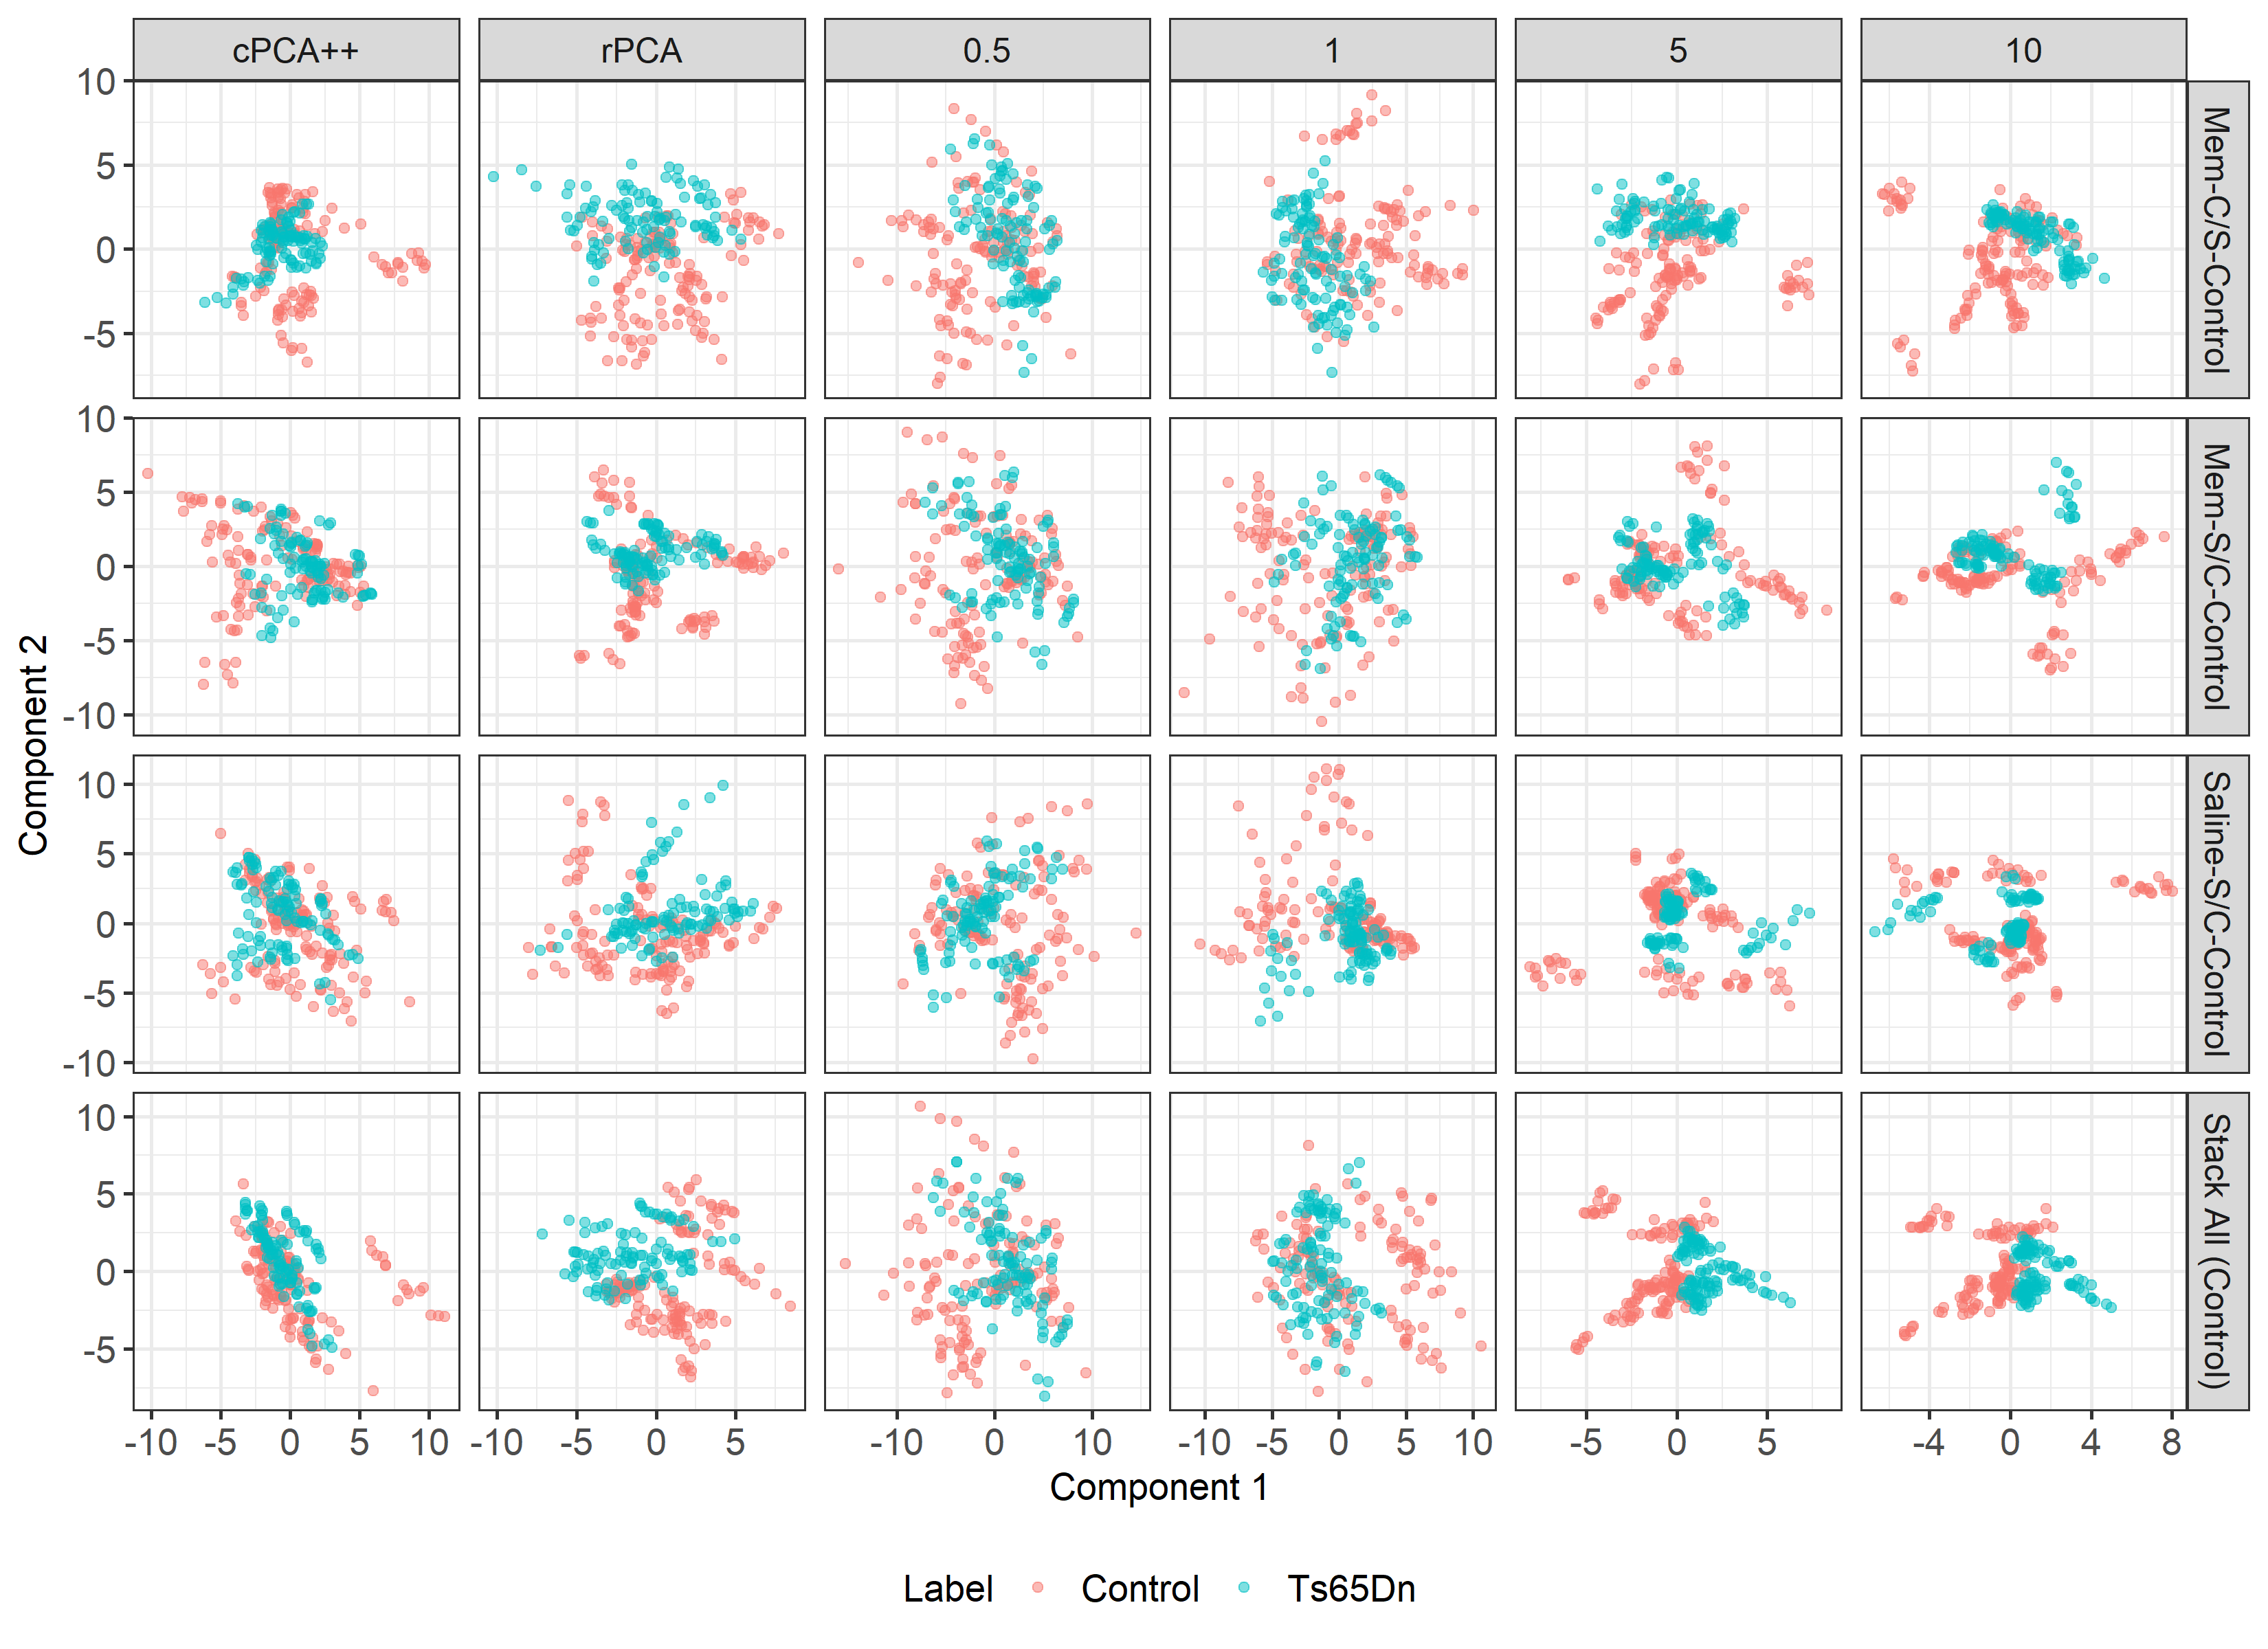
\includegraphics[width = 0.8\textwidth]{figure/Mouse_stack_cpc_rpcControl.png}
	\caption{Mouse Protein Expression Dataset}
	\label{fig:mouse_control_vary}
\end{figure}

\begin{figure}[!ht]
    \centering
	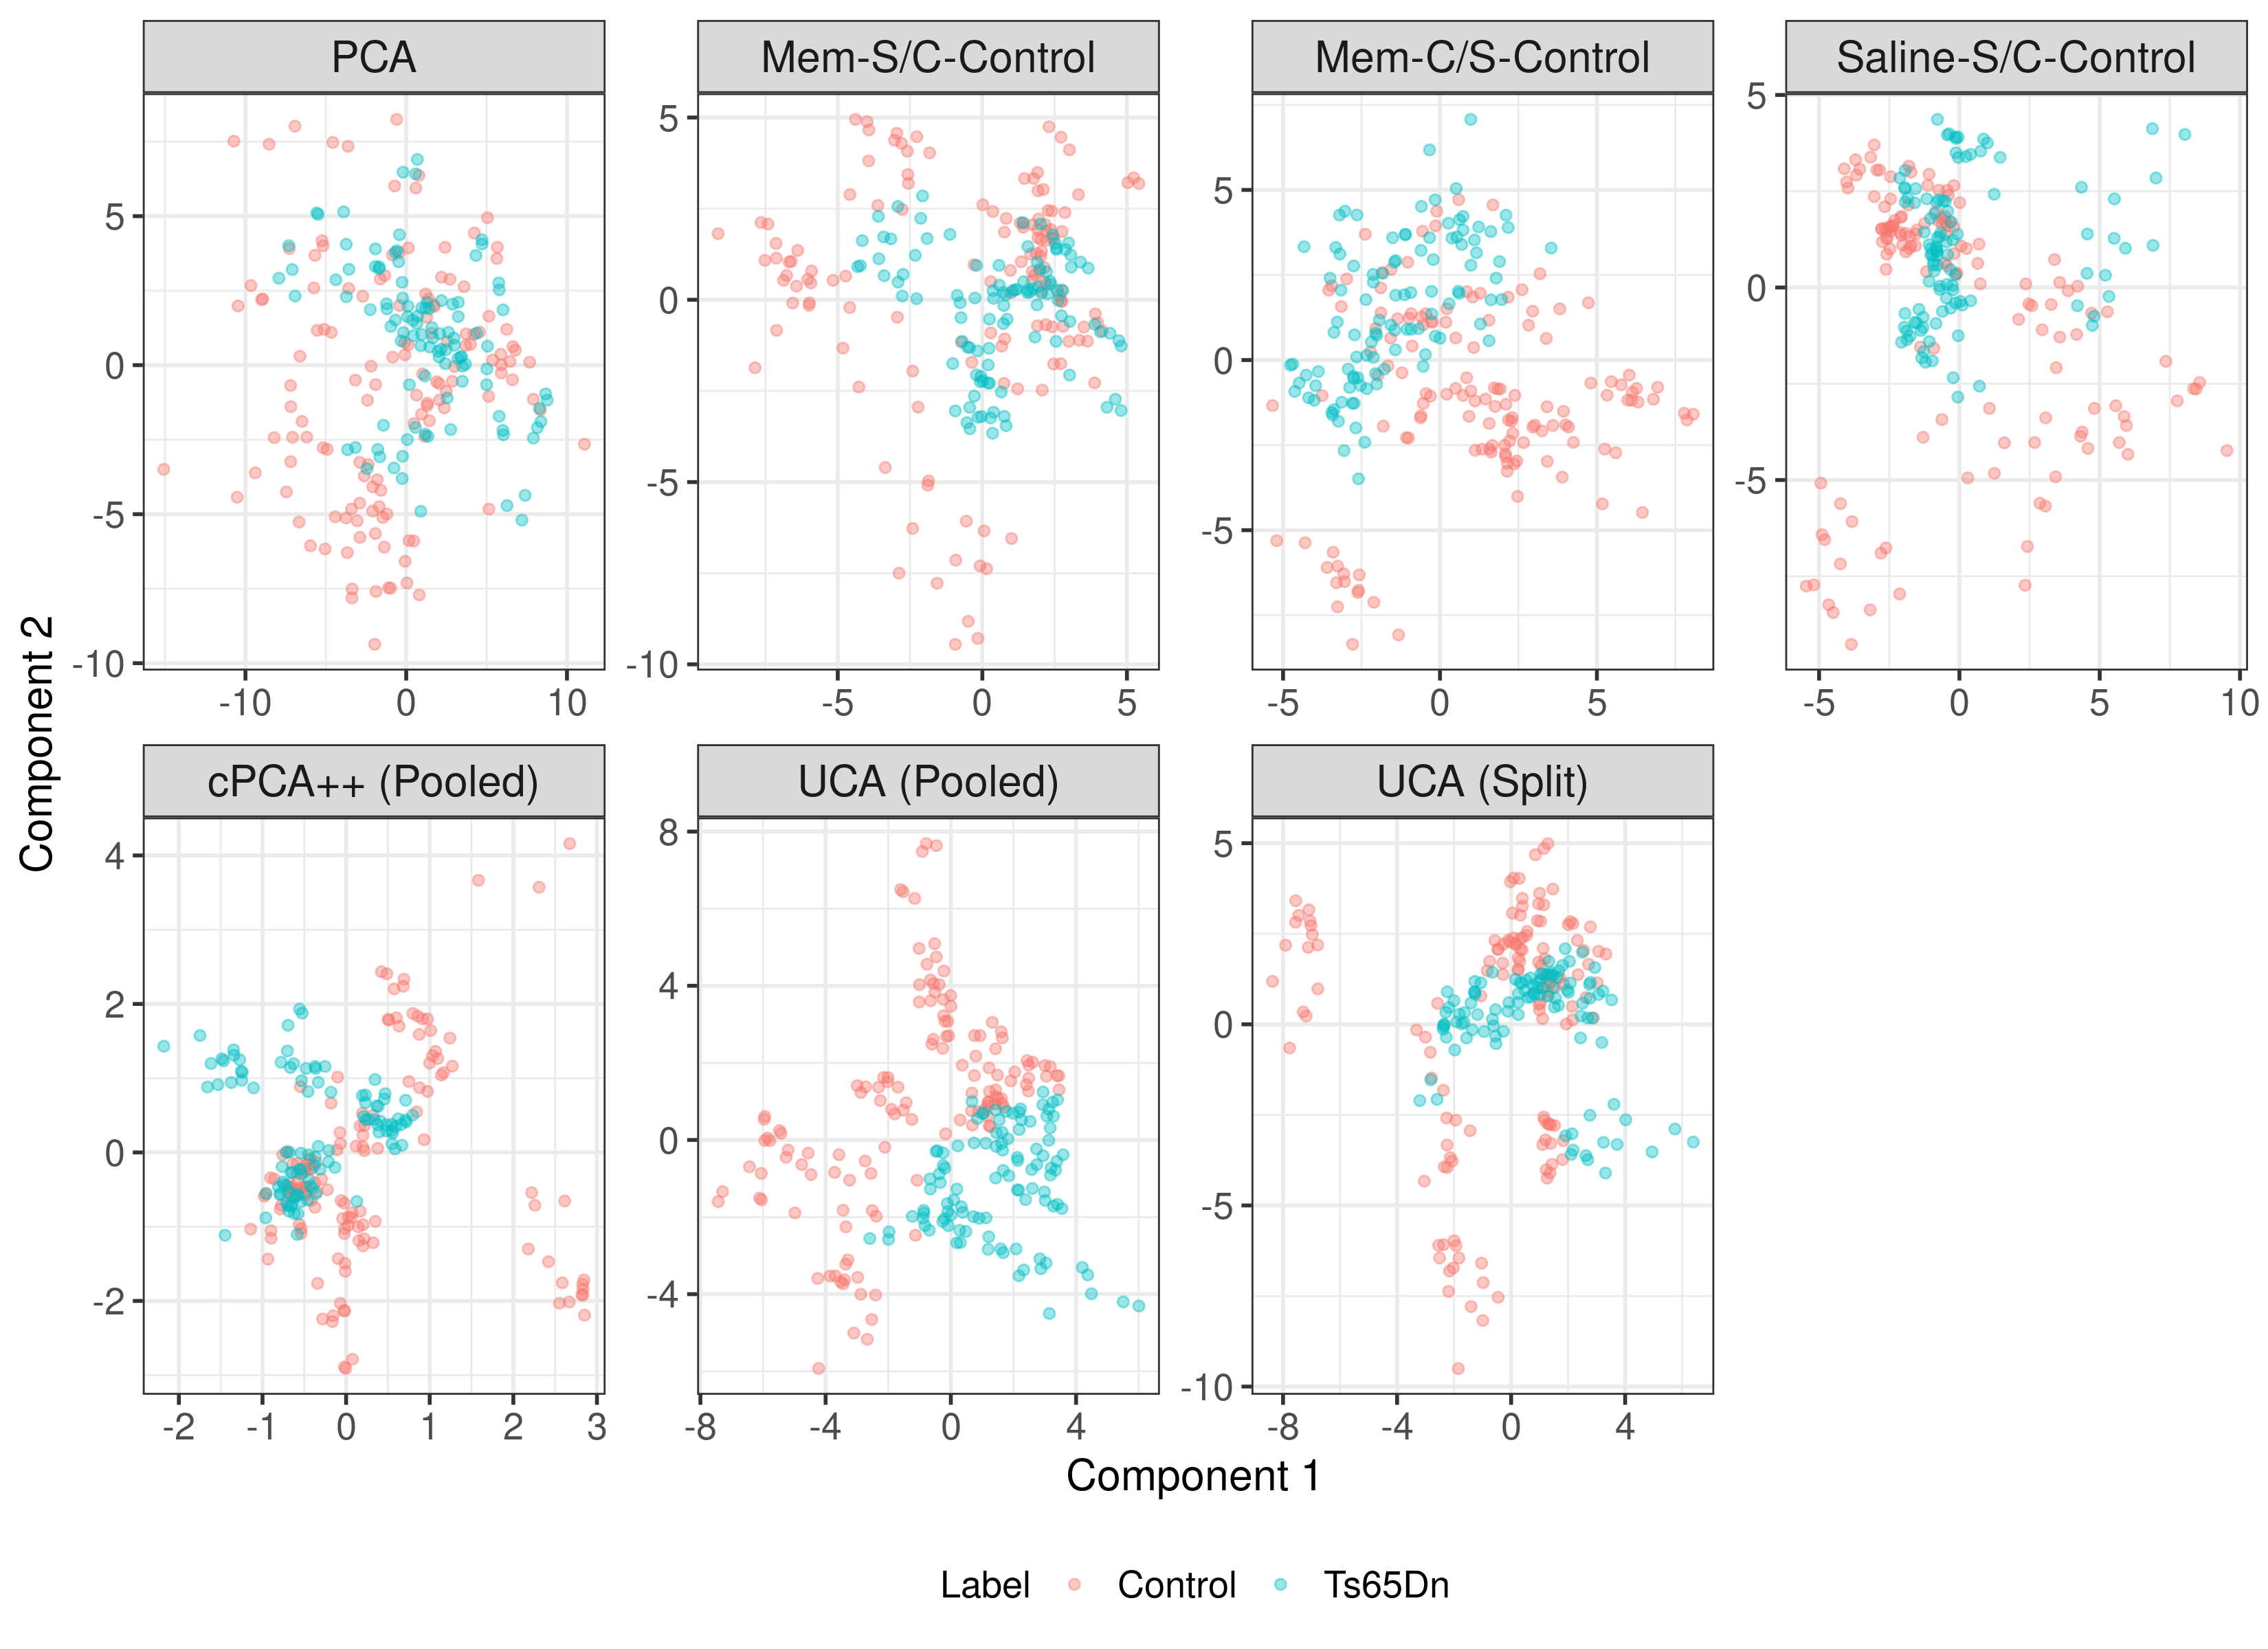
\includegraphics[width = 0.8\textwidth]{figure/Mouse_split_stack_Control.png}
	\caption{Mouse Protein Expression Dataset}
	\label{fig:mouse_stack_control}
\end{figure}

\end{document}



%%% TO DO %%%
% format like Nature communications
% Change captions for mouse and finish mouse results section.
% add caption to KDEF image
% write introduction
% updated results on speed performance in methods section

%%% Things to think about %%%
% an interpretation for $\lambda$
% are our solutions unique? why force v^T Bv  = 1, not 0.25 or 2. does the result give us the same eigenvectors but scaled eigenvalues?
%if you scale the constraint does the estimated v just a scaled version?
%I.e. does it just live in the same space? Maybe the direction wouldn't change
